\documentclass[a4paper, 12pt, oneside]{Thesis}
%%\usepackage[latin1]{inputenc}
\usepackage{amsmath,amsfonts,amssymb,graphicx,setspace,url,verbatim,subfigure,listings} %breakurl
%\usepackage[sort&compress]{natbib} 
%\usepackage[parfill]{parskip}

%\usepackage[english]{babel}

\usepackage[nopar]{lipsum} % for dummy text
\usepackage[american]{babel}
\usepackage[babel]{csquotes}
\usepackage[notes,natbib,isbn=false,backend=biber,authordate,url=false]{biblatex-chicago} 
\usepackage{mdframed}

%\usepackage[showframe,paper=a4paper,margin=1in]{geometry}
%\usepackage[noibid, authordate,backend=biber,doi=true]{biblatex-chicago}  
\addbibresource{thesis_2012.bib}
\DefineBibliographyStrings{english}{%
  bibliography = {REFERENCES},% replace "references" with "bibliography"  for `book`/`report`
}

%%\usepackage[framed,numbered,autolinebreaks,useliterate]{mcode}

% Include any extra LaTeX packages required
%\usepackage[square, numbers, comma, sort&compress]{natbib}  % Use the "Natbib" style for the references in the Bibliography
\usepackage{verbatim}  % Needed for the "comment" environment to make LaTeX comments
%\usepackage{vector}  % Allows "\bvec{}" and "\buvec{}" for "blackboard" style bold vectors in maths 

\usepackage{minted}
\usepackage{fontspec}{
\usepackage{multicol}

\hypersetup{urlcolor=blue, colorlinks=true}  % Colours hyperlinks in blue, but this can be distracting if there are many links.

%\usepackage[pdftex]{graphicx}

\setlength{\parindent}{0in}
\urlstyle{rm}
\hypersetup{linkcolor=black, urlcolor=black, colorlinks=true, citecolor=black}
\usepackage{float}
\usepackage{chngcntr}
\AtBeginDocument{\counterwithin{listing}{chapter}}

\begin{document}

%% ----------------------------------------------------------------
\newcommand{\xten}{\texttt{X10ABOT} }
\newcommand{\reg}{\textsuperscript{\textregistered}}
\newcommand{\lego}{LEGO\reg }
\newcommand{\iic}{I$^2$C }
\newcommand{\includecode}[1]{\inputminted[linenos=true,breaklines=true,baselinestretch=1,frame=lines,framesep=2mm,label=\url{#1}]{c}{#1}}
\definecolor{bg}{rgb}{0.95,0.95,0.95}
\definecolor{hilite}{rgb}{0.95,0.95,0.5}
%\renewcommand\listingscaption{Code Example}
%\renewcommand{\thelisting}{\thesection-\arabic{listing}}


\pagestyle{fancy}
\frontmatter

\begin{titlepage}
\singlespacing
\begin{center}

{\uppercase{The X10ABOT Modular, Extensible, Robotics Platform}}
\mbox{ }\\ 
\mbox{ }\\ 
\mbox{ }\\ 
\begin{center}
A Thesis\\ 
Submitted in Partial Fulfilment of the Requirement for the \\
Degree of Master of Philosophy in Computer Science\\
%in the\\
%Department of Computing\\
%Faculty of Pure and Applied Sciences\\
\mbox{ }\\ 
\mbox{ }\\ 
\mbox{ }\\ 
\mbox{ }\\ 
\mbox{ }\\ 
of\\
The University of the West Indies\\
\end{center}
\vfill
by\\
Rohan Anthony Smith\\
2015\\
\end{center}
Department of Computing\\
Faculty of Science and Technology\\
Mona Campus
%\begin{center}
%Supervisor: Dr. Daniel Coore\\
%August 15, 2012\\
%\end{center}
%\end{center}

\end{titlepage}

\addtotoc{Abstract}
\mbox{ }\\ 
\mbox{ }\\ 
\mbox{ }\\
\mbox{ }\\ 
\abstract{
\begin{center}
The X10ABOT Modular, Extensible, Robotics Platform\\
\mbox{ }\\ 
\mbox{ }\\ 
\mbox{ }\\ 
\mbox{ }\\ 
\mbox{ }\\ 
Rohan Anthony Smith\\

\end{center}
\vfill

We present the architecture and design of a general purpose robotics development kit, called X10ABOT, which aims to facilitate the rapid development of robotic solutions to a wide variety of problems. Robotics kits of this sort are usually aimed at casual hobbyists and children. As a result, these kits usually have severe limitations in the number of sensors and actuators that they can manage. In contrast, X10ABOT is: modular (new functionality can be added through standard daughterboard modules), scalable (up to a maximum of 16 sensors and actuators on each of up to 112 daughterboard modules if implemented on harware with sufficient resources), and extensible (modular software can be added to support new types of sensors and actuators). We have also designed generic ports, capable of handling several types of sensors and actuators. 
We demonstrate the application of the platform to the development of a general purpose robotics kit, using the Arduino development board. In this implementation, we will show how the system would allow its users to readily add extra sensors and actuators to a project, with minimal configuration, and relatively little impact on the pre-existing user code.



\textbf{Keywords:} Robotics; Modular; Extensible.
\newpage
}

\doublespacing
\raggedright
\acknowledgements{
\vbox{}
I would like to acknowledge the support of my close family and friends who served as the motivating factor that propelled me to finish.

I would like to offer my sincere thanks to my supervisor Pr. Daniel Coore, who has provided me with endless guidance and support.  He has been an inspiration in my field and has provided me with insight and vast knowledge to help in the successful completion of this thesis.


Thanks to the Department of Computing, for providing me with the opportunity to further my studies and financial support through the Departmental Award.  

To the members of my research group, I owe many thanks for the drive and motivation in completing my studies.  The weekly meetings are an essential part of providing the momentum to complete.

Finally, this project could not have been complete without the strength and knowledge endowed upon me by God.

\clearpage
}


\dedication{
\vbox{}
This thesis is dedicated to my beloved wife Valene, son Rojé and family. They have been there for me, even when I have all but given up. Thanks for keeping me going.
}

%\thispagestyle{empty}
\tableofcontents
\listoffigures
\mainmatter

\chapter{Introduction} 


\section{Context}
The \xten robotics platform is a general purpose robotics kit that was designed to be a low cost, modular, scalable and extensible option for developing custom robotics projects. The system's intended audience and applications range from simple primary school level robots to more complex creations used at university level robotics competitions and research programs. The \xten kit's focus was to improve upon current general robotics kit standards by providing:
\begin{itemize}
\item Support for potentially hundreds of sensors and actuators.
\item A modular design with pluggable add-on peripheral boards.
\item An extensible software and hardware architecture that easily supports new devices.
\item A low overall cost while achieving all the above listed requirements.
\end{itemize}

Although many general-purpose robotics kits exist, many are either quite limited in the range of models that can be built with them, or demand a high price for their expressiveness. Many of the current robotics kits are designed with a limited number of available ports for attaching sensors and actuators. This is evident in the general purpose LEGO Mindstorms Robotics kit and most of the wheeled platforms like the Boe-bot and the Rug Warrior Pro. %~\parencite{6frompaper}. 
The underlying designs of these kits only partially support scaling, or not at all: one is forced to limit the features of one's robotic designs to operate within this limitation. Inadequate peripheral interfaces can curb creativity and innovativeness, resulting in unfulfilled designs, especially for robotics novices.

The \xten robotics platform is a mix of both hardware and software. The hardware consists of two types of modules, a motherboard and daughterboard. These however can be implemented on a single piece of hardware with a single microprocessor or on their own physically separate hardware modules. For physically separate boards, they are connected via a bus that passes data and instructions between a single motherboard and one or more daughterboards. The daughterboards in turn process these instruction and data and subsequently execute them by applying them to sensors and actuators connected to their respective ports.

There are specialised software components present on each hardware module. The motherboard hosts the user generated program code and the system software that processes it. The middleware is present on both the motherboard and daughterboard, and is responsible for seamless cross-board communication. Finally there is the firmware which is embedded in the daughterboard, this is semi-permanent software that was specialised to interpret and execute instructions passing between the sensors and actuators to and from the motherboard.

\section{Thesis Summary}
Outlined in this thesis are the details of how we progressed from our conceptual ideal product of a low-cost, modular, scalable, extensible robotics kit to transforming these ideals into realistic software and hardware components. These components were modelled and tested using the Arduino embedded development platform. We utilised one or more Arduinos to represent the motherboard daughterboard setup that we envisioned. We also took advantage of the the Arduino software framework which was used to develop the system software, middleware and firmware, all user produced program code would also need to comply with the Arduino software framework.

The outcome of the use of these tools and strategies gave us a system that was able to easily control multiple sensors and actuators in a scalable and modular way while allowing for extensibility.

Listing~\textbf{\ref{code:simpl}} describes a typical code setup for a very simple mobile robot using the \xten framework. All the sensors and actuators were placed on one board (the daughterboard) for this simple implementation. This robot has one actuator (a DC motor connected to an external H-bridge), a force sensor and a pushbutton sensor. The instruction in Listing~\textbf{\ref{code:simpl}} drives the motor at full speed if either the touch sensor records an input or if there is a force on the force sensor above a certain threshold, otherwise the motor will be given the off signal.

 We then further extended the same simple example from Listing~\textbf{\ref{code:simpl}} to show how the \xten framework is able to scale modularly.
 In Listing~\ref{code:simplplus} an extra DC motor and a light sensor were added as a single module. Instructions were then added to activate the new DC motor if there was light intensity above a certain threshold on the sensor. The code example shows that even with the addition of two independent devices, \emph{motor1} and \emph{lightSensor} to the system, it did not affect the existing code but fit seamlessly in the development process.
 

\begin{listing}
		\footnotesize
		\caption{Example of a single controller with a force sensor and a DC motor.} \label{code:simpl}
		\begin{minted}[bgcolor=bg,baselinestretch=1,frame=lines,framesep=2mm,label={Simple Example}]{c}

/**
* Import the necessary libraries for the motherboard, 
* internal daughterboard and the peripheral bus
**/
#include <Wire.h>  
#include <X10ABOT_MB.h>
#include <X10ABOT_DB.h> //Include the internal daughterboard #0 (SELF)

//Initialise the DC motor on daughterboard #0 (SELF), actuator port #1
Actuator motor1(SELF,1);
//Initialise force sensor on daughterboard #0 (SELF), sensor port #1
Sensor force1(SELF,1);
//Initialise force sensor on daughterboard #0 (SELF), sensor port #2
Sensor pushbutton(SELF,1);

void setup(){}
void loop(){
//Continuously check the sensors for a reading
  if(pushbutton.readDigitalB() || (force1.readAnalog()>100)){
    motor1.aB(); //Turn motor1 on by sending LO on pin a and HI on pin B
    motor1.pwm_a(100); //operate motor1 at full power (100%) 
  }else{
    motor1.ab();//Turn motor1 off by sending LO on pin a and pin b
  }
}	 
	\end{minted}
		
\end{listing}


\begin{listing}
		\footnotesize
		\caption{Now we add: A pushbutton sensor to the motherboard (or daughterboard \#0). We also add an extra daughterboard with a light sensor, and a DC Motor} \label{code:simplplus}
		\begin{minted}[bgcolor=bg,baselinestretch=1,frame=lines,framesep=2mm,label={Complex addition to simple example}]{c}
        \end{minted}
        \begin{minted}[bgcolor=bg,baselinestretch=1]{c}
/**
* Import the necessary libraries for the motherboard, 
* internal daughterboard and the peripheral bus
**/
#include <Wire.h>  
#include <X10ABOT_MB.h>
#include <X10ABOT_DB.h> //Include the internal daughterboard #0 (SELF)

//Initialise the DC motor on daughterboard #0 (SELF), actuator port #1
Actuator motor1(SELF,1);
//Initialise force sensor on daughterboard #0 (SELF), sensor port #1
Sensor force1(SELF,1);
//Initialise force sensor on daughterboard #0 (SELF), sensor port #2
Sensor pushbutton(SELF,1);
   
void setup(){}
void loop(){
//Continuously check the sensors for a reading
if(pushbutton.readDigitalB() || (force1.readAnalog()>100)){
    motor1.aB(); //Turn motor1 on by sending LO on pin a and HI on pin B
    motor1.pwm_a(100); //operate motor1 at full power (100%) 
  }else{
    motor1.ab();//Turn motor1 off by sending LO on pin a and pin b
  }
 const byte BOARD2 = 9; //Constant with arbitrary daughterboard address
 //Declare motor on daughterboard #9, actuator port #1
 Actuator motor2(BOARD2,1);
 //Declare force sensor on daughterboard #9, sensor port #1
 Sensor lightSensor(BOARD2,1);
 
//Added extra functionality with a new sensor and a new actuator
//on daughterboard #9 while light is on the sensor, activate motor2
if (lightSensor.readAnalog()>700)
  {
    motor2.Ab(); //Turn motor2 on by sending HI on pin A and LO on pin b
    motor2.pwm_a(50); //operate motor2 at half power (50%)
  }else{
    motor2.ab();//Turn motor1 off by sending LO on pin a and pin b
  }
}	 
	\end{minted}
		
\end{listing}

\paragraph*{Thesis Statement}
\textit{It is possible to design an architecture for a general purpose robotics platform using the Arduino\texttrademark\ microcontroller and supporting software, open-source libraries and tools. It appears that by using a modular, distributed architecture for both hardware and software, it is possible to create a low cost, scalable system with the ability to support hundreds of sensors and actuators. Furthermore, the same API for hardware control that was used to implement the modular and scalable design can be leveraged to allow user defined extensions to hardware interfaces. Finally, all of this can be implemented with only moderate latency penalties (~250-540$\mu$s per digital read/write) .} 


\section{Structure of Thesis}
Chapter 2 explores the design goals of the \xten platform, how the the same principles were being used by other robotics systems and how we applied them for our purpose. 
Chapter 3 describes the design and implementation of the entire platform, the technologies used and how we integrated them to work seamlessly together.
Chapter 4 illustrates the results that will demonstrate the effectiveness of the design strategies we used.
Chapter 5 explores the potential areas for future work and concludes the thesis.

 % \chapter{Introduction}
\chapter{Background and Motivation} % (fold)
\label{cha:background_and_motivation}
%\lipsum[1]~\parencite{modcom}

Robotics development is a continually growing field with a promising future. the
current sate of robotics can be compared to that of the PC industry in its
embryonic years~\parencite{billgates}. Many of the issues that the PC industry faced are redefining
themselves in today's robotics arena. The main ones include high costs, a lack
of common standards and generic platforms. Whenever it becomes necessary to
develop a new robot for a particular task, it is often necessary to build
it from scratch. This is because there are few general purpose platforms that meet
all the needs of the typical robotics engineer, student and hobbyist~\parencite{r2p}. The
``killer app'' for the robotics industry will be a platform that can address these issues
and thereby create a broader adoption of robotics technology. As with the
computer industry, one of the main markets that utilise robotics is education.
Robotics is used to teach students of all ages and levels on topics ranging from
science to social skills~\parencite{kramer}. General Purpose Robotic kits are one of the many
`edutainment' methods that are developed. These kits provide the user with the
ability to build robots for a large range of applications.

An increased interest in robotics and robotics development has fuelled 
the search for a robotics platform that will be useful for schools and the 
typical hobbyist. There has been research into finding a suitable
platform that is flexible, inexpensive, extensible and capable of handling
projects of varying complexities~\parencite{bot-mate}. Popular kits exist that meet some of
these characteristics. For instance, the Lego Mindstorms\texttrademark  robotics
kit is one of the most popular robotics platforms that can achieve many of these
requirements. It however achieves a few of them through unconventional
`hacking' of the platform, or by purchasing third party equipment. This is not
always easy to accomplish for beginner developers. This project will outline
the means by which the \texttt{X10ABOT} robotics platform provides for these
specifications seamlessly through the features built into its design.

The \texttt{X10ABOT} robotics platform  was designed from the ground up by integrating useful strategies
found in other general purpose and custom robotics kits. This along
with other innovations form the \texttt{X10ABOT} robotics platform's
architecture. We accomplished this by focusing on achieving the combined goals of modularity, 
extensibility and scalability while maintaining a relatively inexpensive cost.

The motivating factors for this project extended from the need for involving
robotics in education. ``Studies show that robotics generates a high
degree of student interest and engagement and promotes interest in math and 
science careers .  The robotics platform also promotes learning of scientific 
and mathematic principles, through experimentation''~\parencite{barker}.
The  inclusion of robotics in a school curriculum has been
shown to improve performance in STEM subjects~\parencite{school}. 
Robotics development allows for students to apply practical techniques to complete tasks and 
to solve scientific problems. The result or response from their work is
immediately observable through the physical response of the robot. In addition,
robotics  presents a `fun factor' that attracts young people.
To adequately utilise robotics as a viable educational platform, certain hurdles 
that were being faced had to be overcome. This lead to the creation of the \texttt{X10ABOT} robotics
platform. This project was aimed at creating a platform that could 
adequately provide a full featured robotics framework for students, all at a
price lower than the current market price for a full featured robotics kit.
This would further assist in the the commoditisation of robotics kits and subsequently
increase the possibility for activities such as robotics competitions between schools.
Other driving motivations for the project included the creation of a platform that
would provide a flexible starting point for other robotics research projects. The kit
would also be useful enough for hobbyist users who were interested in robotics
and automation, the \texttt{X10ABOT} robotics platform would be an attractive tool to be utilised in their projects.

\section{Similar Projects} % (fold)
\label{sec:similar}
We researched the structure of several robotics research projects and commercial robotics kits and identified a number of design objectives that were useful for a general purpose architecture. We aimed at creating a robotics framework that was able to support more sensors and actuators than most of the popular robotics kits, it had to support most of the common off-the-shelf sensors and actuators and yet be easy to use without limiting creativity. 

%Mention in the field kits like Tetrixx
We reviewed many types of robotics projects and came across a few interesting concepts. The following projects were encountered at varied intervals between design and completion, they both influenced and validated the design decisions made in the \xten project. We will review a few of them and present an overview of their architectures. 

The Tetrixx robotics project was developed in the late 1990's. It sought to overcome the issue of expandability being faced by its contemporaries such as MIT's 6.270 board and Handyboard~\parencite{handy} projects. To overcome this limitation, the Tetrixx project employed specialised sensor and actuator expansion boards connected over a bus. The bus supported up to 64 expansion boards and allowed it to scale to far more peripherals than limited by the connectors from one single controller~\parencite{tetrixx}. This was one of the first systems that influenced the expansion board concept used in our project.

Another interesting robotics kit project was the LEGO Mindstorms NXT robotics development platform. This is a very popular robotics kit among schools and hobbyists. It has three actuator ports and four sensor ports on its controller unit. Additional sensors and actuators can be added either by pairing with another controller or by purchasing third party multiplexing devices that allow multiple peripheral devices connected to one port. The port design is quiet extensible with numerous analogue and digital I/O pins and an \iic bus to support even very complex devices. The Mindstorms kit has the distinct advantage of having a very active community of developers who have worked to create a large set of programming interfaces that can be used to write robotics applications for the platform. These include compilers for some of the most popular programming languages such as, C, Java, Python, Ruby, Ada, Lua and Matlab. The Mindstorms kit represented to us a very modern architecture and served as a standard by which we measured a lot of our innovations. The Mindstorms kit however lacked the scalability we required, its other architectural attributes, however, were emulated in our design. It was also advantageous that most of the system was open sourced. We modelled our sensor and actuator ports after a similar design, we also took note of the software architecture and structured the \xten to be able to facilitate a virtual machine type plugin that can interpret the Lego NXT bytecode. We started work on this but realised that the magnitude of effort required was beyond the scope of this thesis.

We explored the architecture of the Hannibal Hexapod robotics project that had a commendable capability of managing the input and output signals for over one hundred (100) physical sensors and actuators~\parencite{hannibal}. The Hexapod robot controller is based on the Subsumption Architecture and is fully distributed across eight(8) onboard computers: one each for the main controller, the robots body and each of its six legs. All these modules are connected via an \iic serial communication bus. These components were the realisation of the Hannibal Hexapod's design requirements of being scalable, modular, flexible, robust and adaptive. The Hannibal project greatly influenced the use of an \iic peripheral bus as the central communication line on a distributed system of robotic components. This seemed to have aided in the management of a large number of sensors and actuators. Since scalability was a desired attribute, we adopted this approach.

We also explored the architecture of the Rapid Robot Prototyping(R2P) project that shared many of the design objectives that were outlined for the \xten architecture. R2P's design goals were to be an inexpensive, open source, modular architecture for rapid prototyping of robotic applications~\parencite{r2p}. Similar to the \xten, this architecture was aimed at students and hobbyists creating robotic applications on low powered microcontrollers. The architecture was built around a distributed system of modules communicating over a high speed serial data CAN bus. It emphasises its plug and play capability by providing ports on each module to support daisy-chaining of multiple peripheral boards. On the software aspect, the R2P has embedded firmware on its peripheral modules to act as a Hardware Abstraction Layer(HAL) to encourage modularity. On the main controller, it implemented a Real Time Operating System(RTOS), a publish/subscribe middleware and a Virtual Machine that supports an embedded scripting language. The R2P system was encountered in the post-design stage of the \xten project. It however validated a very large portion of the design of our architecture. The R2P system was very similar to \xten only differing in a few areas e.g. a CAN serial bus was used instead of \iic serial bus. 
%
%
These examples influenced and validated some of our design decisions for the components of the \xten architecture. We chose a combination of the best features of these technologies which we found to improve modularity, scalability and extensibility and combined them to construct our framework. 

%{TABLE HERE}
%Table showing comparison of robotic platforms and a measure of their
%capabilities





\subsection{Modularity} % (fold)
\label{sub:modularity}
Modularity in the design of a robotics kit architecture defines the capability to incrementally add fully independent sub-systems to a robotics project without significantly modifying the existing configuration. According to Oraw and Tinder~\parencite{mars}, ``The modularity of a robot is demonstrated by its expandable intelligence. Sensory modules that implement the robot's data protocol can be plugged into the system without reprogramming the original components''. They also mention that the key to modularity is the use of peripheral modules. These were just a few of the design decisions made to satisfy our requirement of a modular architecture. 

We chose to use a distributed system as a part of the architecture. This allowed for the control of the overall system to be shared across multiple independently operating modules. These modules operate efficiently because there is very minimal usage of shared resources, this is because each module is usually self sufficient and simply passes information back and forth between itself and the main controller over the data bus. In a centralised system which is dependent on one main processor, management of peripherals can become complex when handling a large number of modules. The controller's resources and connections are limitingly finite and there may be contention for these resources which may even prevent the inclusion of additional modules without the need to remove a previous module or somehow hack the system.  Using a distributed system not only reduces complexity but it also allows for changes to be made across the entire architecture without affecting the existing setup~\parencite{avcithesis}.

A subsequent advantage of a modular architecture is software and hardware reuse, and rapid prototyping. Peripherals can be incrementally added to build more complex projects and subsequently reduce the overall cost of development~\parencite{modcom}. Different functions of the system can be delegated to independent and specialised modules. The aim was to simplify the control problem by decomposing the global task into local tasks for the robot's subsystems~\parencite{rdk}. This reduces the computational load on the main processor by delegating the majority of the low level sensor and actuator processing to sub-modules. 

Another common practice that many robotics architectures employ is the inclusion of peripheral sensor and actuator boards in their design. This can be seen in the Tetrixx project~\parencite{tetrixx} and numerous other robots built around a distributed processing architecture. Peripheral boards are secondary computational units that are responsible for low level control operations. These peripheral boards interpret and execute data and control commandscommunicated between the main controller and the board's sensors and actuators. They are connected to a peripheral bus which will be able to uniquely identify each module along the communication line. 

The peripheral bus that we selected supports up to 112 modules that can facilitate advanced robotics projects. Another requirement of the peripheral bus is high bandwidth that will be able to accommodate the possibility of a large number of active peripherals in a single session. We designed peripheral boards, named daughterboards that support sensors and actuators connected to the main controller over a fast, addressable serial peripheral bus. The daughterboards interact with the main controller board through a master-slave relationship. In our implementation, there exists just two types of components, the motherboard and daughterboards. Both type of modules have processors designated for their particular tasks, of which the motherboard may be required to be more powerful.


 
% subsection modularity (end)

\subsection{Scalability} % (fold)
\label{sub:scalability}
Robotics kits that can support projects of varying complexities should have the ability to support as many sensors and actuators as may be required for a complex robotics project. A robotics project can range from robots that complete simple tasks that require one or two sensors and actuators to robots that manage tens of sensors and actuators necessary to complete their task. As the complexity of a robotics project increases, generally, so does the number of peripherals required to complete the tasks. Projects that may solve reasonably technical tasks will sometimes have to improvise by finding creative ways to use available resources, however there may be times that the scale of the project requires a large number of sensors and actuators to adequately perform the task. Robots that are known for using a large number of sensors and actuators are usually ones that try to replicate animal or human ability. One such example is the Hannibal Hexapod Robot. Hannibal receives a tremendous amount of sensor  information while continually controlling its almost 20 servo motors.  The spider-like robot has over 60 sensors of different types~\parencite{hannibal}. Other types of robots that utilise many sensors and actuators include robotics arms, full humanoid robots, and animal replicas like MARS: the Modular  Autonomous Robotics Snake~\parencite{mars}. In all of the above examples, the supporting architecture facilitated the inclusion and efficient management of a significant number of sensors and actuators.

 We wanted to ensure that the cost of scaling was not prohibitive and that the developers would save on both time and money when implementing their large-scale robotics project. A distributed robotics architecture is key to decreasing the cost-to-scale factor. In a distributed system, the processing is shared between a central processing unit or a motherboard and numerous specialised modules. These modules are usually focused on doing simple tasks and therefore will not require complex hardware or devices to accomplish them. This can therefore allow them to to be inexpensive and simply connect to the motherboard to report the results of its computations and fetch data on request.


 We needed a robust architecture that provided more than just an increase in connection points for sensors and actuators. It is critically important that there is adequate hardware and software support for the increase in additional devices. Proper power management is very important when managing tens to hundreds of sensors and actuators. These devices can behave erroneously or simply fail to perform if they are not supplied with adequate power. It is also very important to place electrically noisy and high powered devices on separate power sources. This is especially true with motors and sensitive, low powered electronics should never share the same power source. This can electrically damage sensitive components of a controller and render the robot unusable. It is also necessary that the system be sized for its maximum power requirements and a capable power source selected. Under-powering a robot can also cause unpredictable results. Sometimes it may even be necessary to have multiple power sources on a robot that are adequately isolated. Our scalable architecture took these requirements into consideration.

Another requirement that may be easily overlooked is a structured and organised wiring and connection system. A robotics project can become increasingly difficult to develop if there is a web of wires and connections attached to the dozens of devices that may be present on a robot. A design that will mitigate this issue is the use of a distributed system supported by a main bus with an addressable serial data connection. If the architecture is designed with a single peripheral bus as its communication backbone which connects all devices, most of the wiring can be placed in a single organised package. The advantage of using an addressable serial bus is that these usually utilise very few connection lines. They also allow for new modules to be daisy chained onto each other. Any addition of a new set of sensors or actuators will simply equate to physically plugging a single set of wires from one module to another.

%Scalable: Support for multiple sensors and actuators.



\subsection{Extensibility} % (fold)
\label{sub:extensibility}
A truly extensible robotics system permits future addition and support of new sensors and actuators which might not have been included in the initial design. Extensibility of a robotics kit provides developers with the freedom to define the hardware configuration with respect to the available types of sensors and actuators~\parencite{rdk}. A robotics kit may never be able to guarantee support for all types of sensors and actuators, but a truly extensible architecture will provides the means for developers to enable support for their particular hardware. 

We used a middleware architecture to hide the low-level details of interface between the components that make up the \xten architecture. This level of abstraction allowed for an interface between the main controller and the sensors and actuators which supported a high level definition of their operations. We saw this technique applied across numerous other platforms, this structural design is referred to as robotics middleware. ``Robotics middleware provides functionality that is to be used and extended by the roboticists. Therefore, the tools provided by the middleware layer have to be capable of extending the robot's functionality in order to be able to cope with its growing capabilities~\parencite{advanced}." There are a variety of ways to practically achieve extensibility through middleware but the general idea is to devise a method of allowing communication between the software on both sides of the middleware. This further abstracts the hardware interaction to the developer. Defining new hardware is now done through a configuration system and the middleware communicates information to and fro without exposing the communication protocol between the source and destination. This further hides any complex hardware setup and presents a flat structure even on a distributed system.
Our system was designed to support as many types of sensors and actuators as possible. To achieve this, we had to find a common denominator for all sensors and actuators. Sensors and actuators have many requisite hardware technologies that need to be supported. We realised that these technologies were subsets or a combination of a finite set of operations. Technologies such as pulse width modulation, hardware interrupts, digital input/output and analog input are just some of the basic ones used by most sensors and actuators. We determined that if we could define this complete set of hardware operations, we could control most if not all sensors and actuators. This would allow extensibility to currently existing and possibly new types of sensors and actuators.
%Extensible: Permit Customized commands for peripherals



% subsection extensibility (end)

\subsection{Economics} % (fold)
An important requirement that will permit wider adoption of the robotics kit is ensuring that the kit's cost and its cost to scale are kept relatively low. The cost of electronics is a decreasing function of time, however these prices are not always instantly obvious in the field of robotics. It is almost an accepted fact that robotics is an expensive field, the prices of robotics kits range from hundreds to thousands of U.S. dollars. This is a major point of restriction, robots are expensive and often beyond the resource of many persons and even universities and organisations who want to delve into the field of robotics~\parencite{vr}. In order to make a robotics kit that will be an attractive option for hobbyist roboticists and school programs even as low as the elementary school level, it has to be available at a competitive price point. A very popular platform for doing robotics is the Arduino development board which at the time of this publication ranged from U.S. \$30 to \$70. The Arduino development board is not specialised for robotics but has all the major tools necessary to build a functional robot if the developer is skilled in electronics. It is also one of the most popular development platforms at robotics competitions.
The Arduino board also has a distinct advantage of being open-source. This gives the developer the advantage of having access to free software upgrades and longer hardware support. Being open-source also means that a skilled developer will be able to make modification to the system's code and even build their own hardware replica. These advantages can mean significant saving if a solution can be accomplished by the developer instead of purchasing an upgraded version or proprietary hardware.

%Inexpensive: Relatively low initial cost andd cost to scale
\label{sub:economics}

% subsection economics (end)

% section design_objectives (end) % \chapter{Background}
\chapter{The \texttt{X10ABOT} Architecture, Design and Implementation}% (fold)
\label{cha:the_x10abot_architecture_design_and_implementation}


In this chapter we describe how we used the design strategies which were introduced in the background chapter. We extracted the most compelling features and combined them to crate a modular system with the following components which comprise the \xten architecture:
\begin{enumerate}
\item The Motherboard
\item The Daughterboard
\item The Peripheral Bus
\item Input and Output Ports
\item The Motherboard Library
\item Daughterboard Firmware
\item The Middleware
\end{enumerate}

%\section{Physical Setup} chapters should represent compoents of the system

% Chapter 3

%%Impact or influence of the design decisions and how they were implemented
The \xten 's main architectural features that were decided on were modularity, scalability and extensibility. It was also important that we kept the cost of implementation relatively inexpensive. These attributes represented common design patterns observed over a number of robotics projects, either for custom robots or as a part of the architecture for general purpose robotics kits. We designed a system which comprises of components which realize one or more of the design requirements.

%User friendly:  Usable primary school to  graduate level roboticists
\newpage
\section{The Architecture} % (fold)
\label{sec:the_architecture}
Based on the design requirements listed in the previous chapter, we created an architecture that captures all the previously listed features without making any significant compromise on any of those aspects. The \xten architecture meets all the previously outlined requirements at both the hardware and software level. It is comprised of a motherboard, the main central controller and the head of a distributed system of peripheral sensor and actuator boards called daughterboards that carry out a standard set of computations synonymous to a thin client, all connected across the central peripheral bus. The motherboard coordinates and controls all operations on the entire system and all operations are either initiated or terminated at the motherboard. The motherboard hosts the main program for the robot application, the middleware and the extensible libraries to support various types of sensors and actuators. Each daughterboards is equipped with firmware to interpret and execute instructions given to it by the motherboard. It also provides multi-faceted sensor and actuator ports that can support a broad range of sensors and actuators. 

\begin{figure}[h]
  \begin{center}
    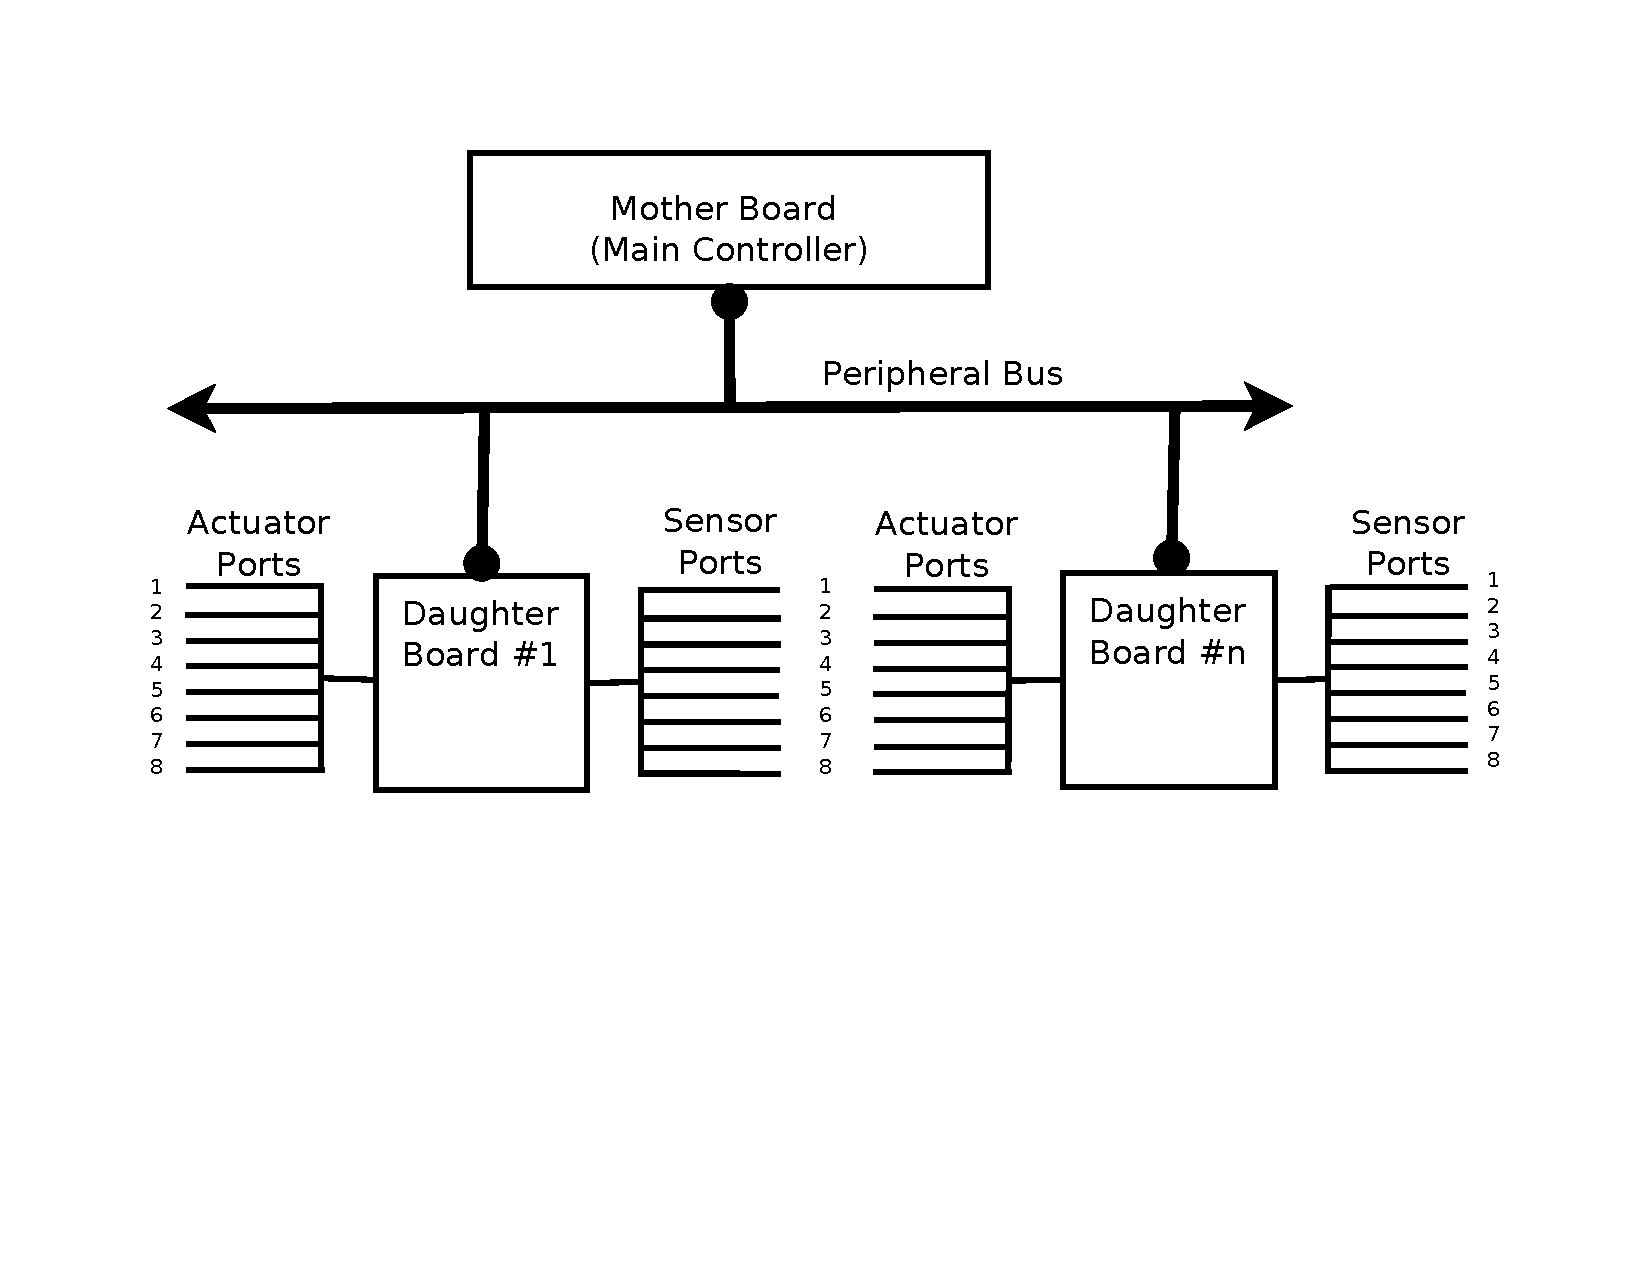
\includegraphics{Figures/system_block_diagram.pdf}
    \caption{The components of the \xten Architecture}
  \end{center}
\end{figure}

\subsection{The Hardware Architecture} % (fold)
\label{sub:the_hardware_architecture}
The hardware aspect of the \xten framework consists of three major components. These are the motherboard, daughterboard and the peripheral bus which connects them all. Below we will describe in detail how each component functions and how they relate to each other in accomplishing the goals of the architecture.



	\subsubsection{The Motherboard} % (fold)
	\label{ssub:the_motherboard}
	The motherboard is a physical component of the robotics platform and operates as the single central processing unit. it controls the flow of data and instructions across the entire \xten architecture. All robot control instructions written by the robotics developer are hosted on the motherboard. The instruction logic is processed on the motherboard, however the actual sensor or actuator operations are dispatched to daughterboards as micro-code instructions. These microcode instructions are then subsequently interpreted and their operations executed by sensors and actuators across the entire system. As the main computational entity in the \xten architecture, the motherboard is responsible for executing most of the decision logic, heavy computing tasks, actuating the output devices and interpreting information from input devices based on its preprogrammed set of instructions.
The motherboard acts as the head of the distributed system of peripheral boards. Sensors and actuators are hosted by daughterboards which are connected to the motherboard via the peripheral bus. 
 
	% subsubsection the_motherboard (end)
	
	\subsubsection{The Peripheral Bus} % (fold)
	\label{ssub:the_peripheral_bus}
	
	\begin{figure}[h]
	  \begin{center}
	    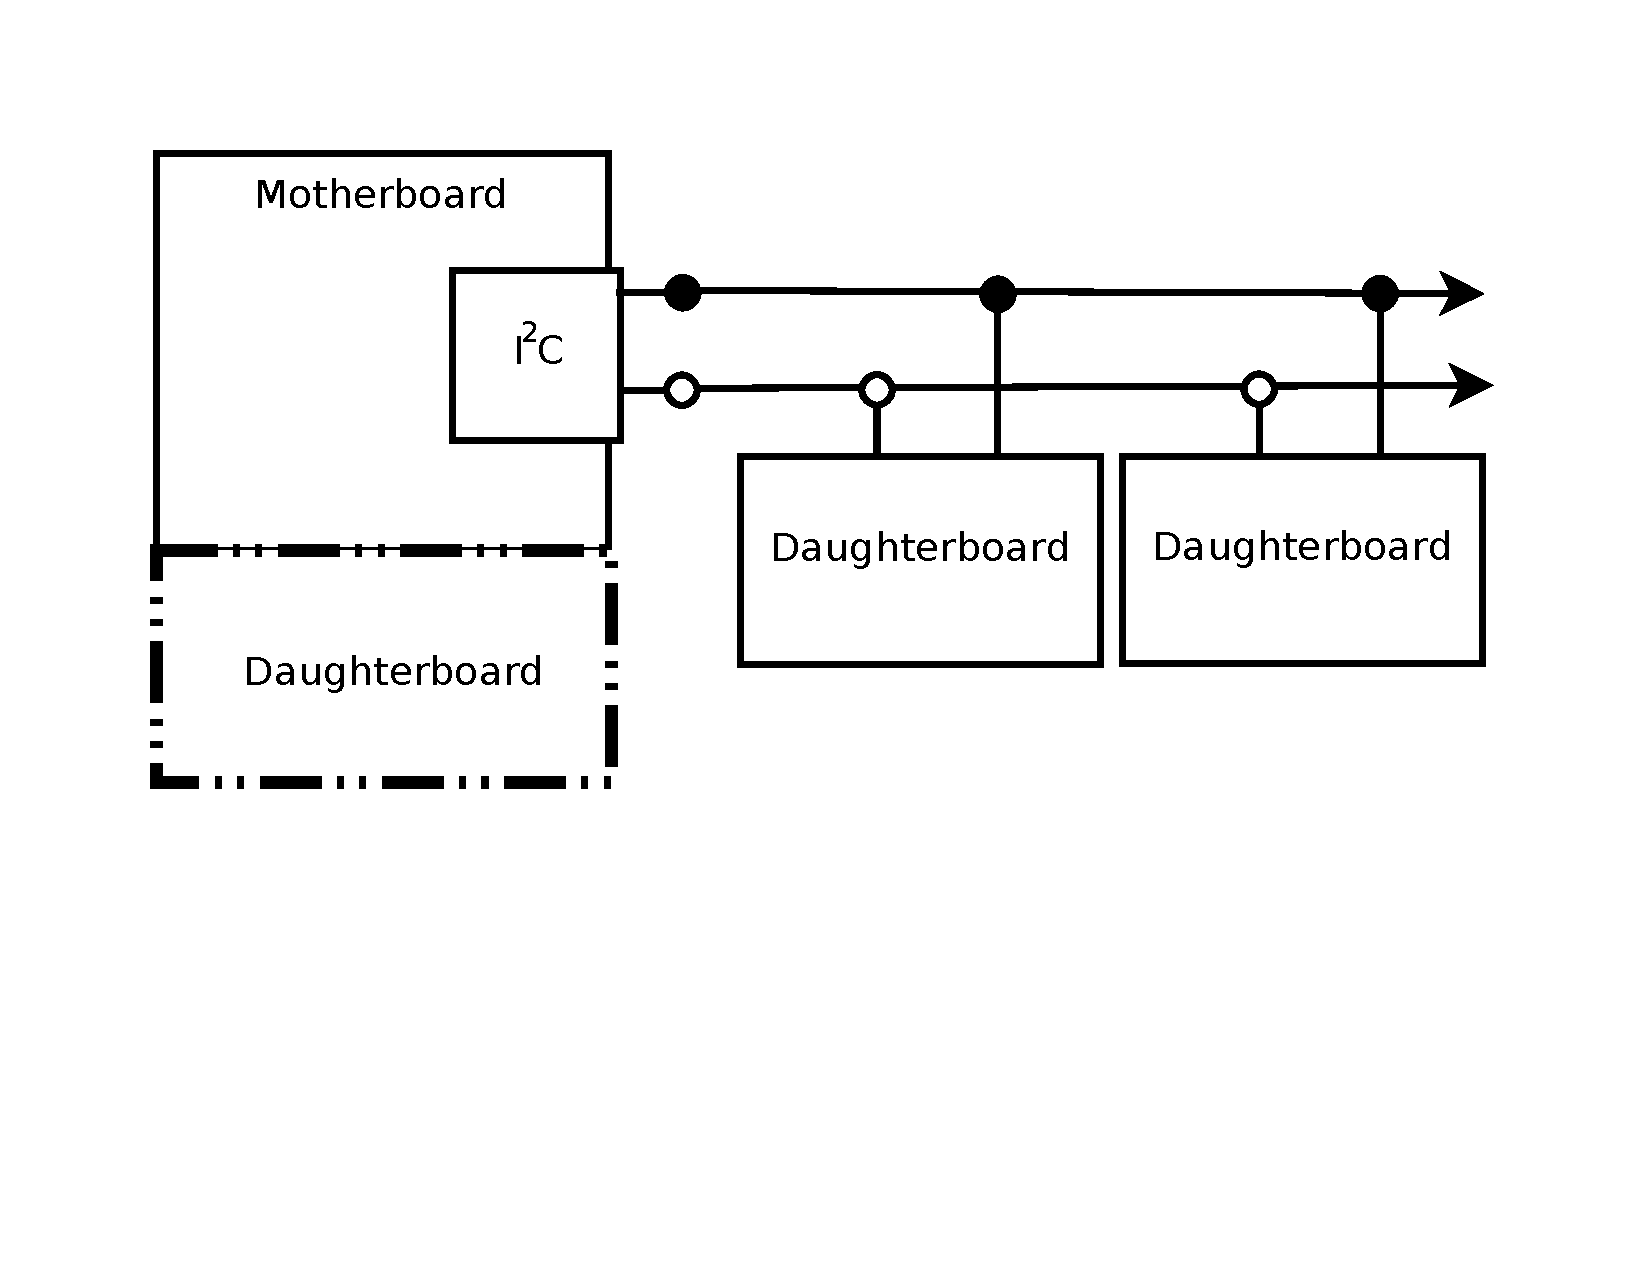
\includegraphics[width=1.0\columnwidth]{Figures/pbus.pdf}
	    \caption{The serial communication peripheral \iic bus}
	  \end{center}
	\end{figure}
	
	The Peripheral Bus is the central medium that connects the motherboard to one or more daughterboards and facilitates the communication of data and instructions between them. The peripheral bus is implemented using the \iic serial communication protocol. \iic is a multi-master, addressable slave, two wire bus serial protocol. It supports up to 112 uniquely addressable devices per bus (128 minus 16 reserved addresses), 8-bit oriented, bidirectional data transfers can be made at 100 Kbits/s in the Standard-mode, 400 Kbits/s in the Fast-mode, 1 Mbits/s in Fast-mode Plus, or up to 3.4 Mbits/s in the High-speed mode \cite{indec}. While operating in its standard-mode, the I2C bus can be as long as 9 - 12 feet without any significant noise interference \cite{nonoise}. This distance is quiet sufficient for a robotics kit where the peripherals are not usually more than 3 feet away from the controller circuit. As such, I2C provides a low-cost solution for interconnecting large numbers of devices operating at relatively slow speeds, such as sensors or other external devices connected to a microcontroller \cite{again}. A number of robotics projects implement this method of data communication, including the popular NXT LEGO Mindstorms Kit, ISocRob, and the Hannibal hexapod autonomous robot \cite{nuffadem}.
	
	% subsubsection the_peripheral_bus (end)
	All communication on the \iic bus is initiated by the bus master or, as in our case, the motherboard. This is not suitable in all situations, e.g.: when a sensor detects an input that needs to be processed immediately. Even if all the daughterboards are periodically polled, the elapsed time may cause the sensor data to become invalid or ineffective. That is why we utilized the multi-master capability of a the \iic peripheral bus to accomplish arbitration. \iic inherently supports collision detection and bus arbitration, bus arbitration refers to a portion of the protocol that ensures that when multiple masters try to control the bus simultaneously, it allows only one master full control of the bus while queuing the prospective master without any corruption or dataloss\cite{nxpi2c}. The motherboard has primary control over the peripheral bus but periodically gives up the control to any daughterboard that wants to gain temporary bus-master status. The capabilities given to a daughterboard that has claimed bus-master status is limited. Daughterboard which claim bus-master status can only communicate with the motherboard, there is no daughterboard-to-daughterboard communication. The daughterboard cannot request data from the motherboard, it can only transmit its own data.
	The peripheral bus allows for easy connection of additional devices because they can be daisy-chained onto each other reducing the need for extensive and confusing wiring. Since the peripheral bus is an \iic bus, it is compatible with ``non-daughterboard'' \iic compatible devices. The framework was designed to accommodate sensors and actuators as specialized, single device daughterboards. This was also a method of ensuring maximal extensibility.
	
	There is one exception to the use of the \iic bus as the main peripheral bus, this involves the use of an internal daughterboard. We will expound on this concept in the next section.
	
	\subsubsection{The Daughterboard} % (fold)
	\label{ssub:the_daughterboard}
	The daughterboard is the secondary computing device in the \xten robotics architecture. It hosts all the sensors and actuators that carry out the tasks of each robotics project. Although the daughterboard is a second tier processing component in the X10ABOT architecture, its operation is not trivial. The daughterboard is given the major task of interpreting instructions sent from the motherboard over the peripheral bus and executes them with sensors and actuators. Sensors and actuators are connected to sensorand actuator ports respectively and respond to the assertions placed upon them by the daughterboard. Daughterboards carry out simple low level operations and won't require a significant amount of processing power. There are however a few basic features that every daughterboard must possess. All daughterboards must be able to communicate over an \iic bus and do basic digital and analogue input and output. These features are very common in most microcontrollers and can be implemented without a significant cost or effort.
	As a member of the peripheral bus, each daughterboard must possess a unique address that the developer is aware of, it also should have knowledge of the motherboards address. All motherboards will have the same address since only one motherboard is allowed on the peripheral bus at a time. A daughterboard will need the motherboard's address whenever it has time critical data that needs to be sent to the motherboard. Using bus arbitration, the daughterboard tries to temporarily claim the bus-master role in order to quickly pass its data to the motherboard, it would then immediately switch back to its slave role.
	\subsubsection{Internal Daughterboard} % (fold)
	\label{ssub:internal_daughterboard}
	
	% subsubsection internal_daughterboard (end)
	On a typical motherboard circuitry, the only external IO pins that are generally utilized are SCK and SCL that operate the \iic protocol. This leaves a large number of unused IO pins that could have otherwise been used for some kind of operation. We then came up with method for utilizing these extra resources without breaking design of the architecture. We design a virtual, internal daughterboard, that uses the same microprocessor and physical board as the motherboard. This internal daughterboard is assigned with address number zero(0). All its data and instructions are communicated using direct parameter passing instead of across the peripheral bus. This particular exception is abstracted by the middleware~\ref{ssub:middleware} and is totally hidden from both the motherboard and the internal daughterboard.
	
	\begin{figure}[h]
	  \begin{center}
	    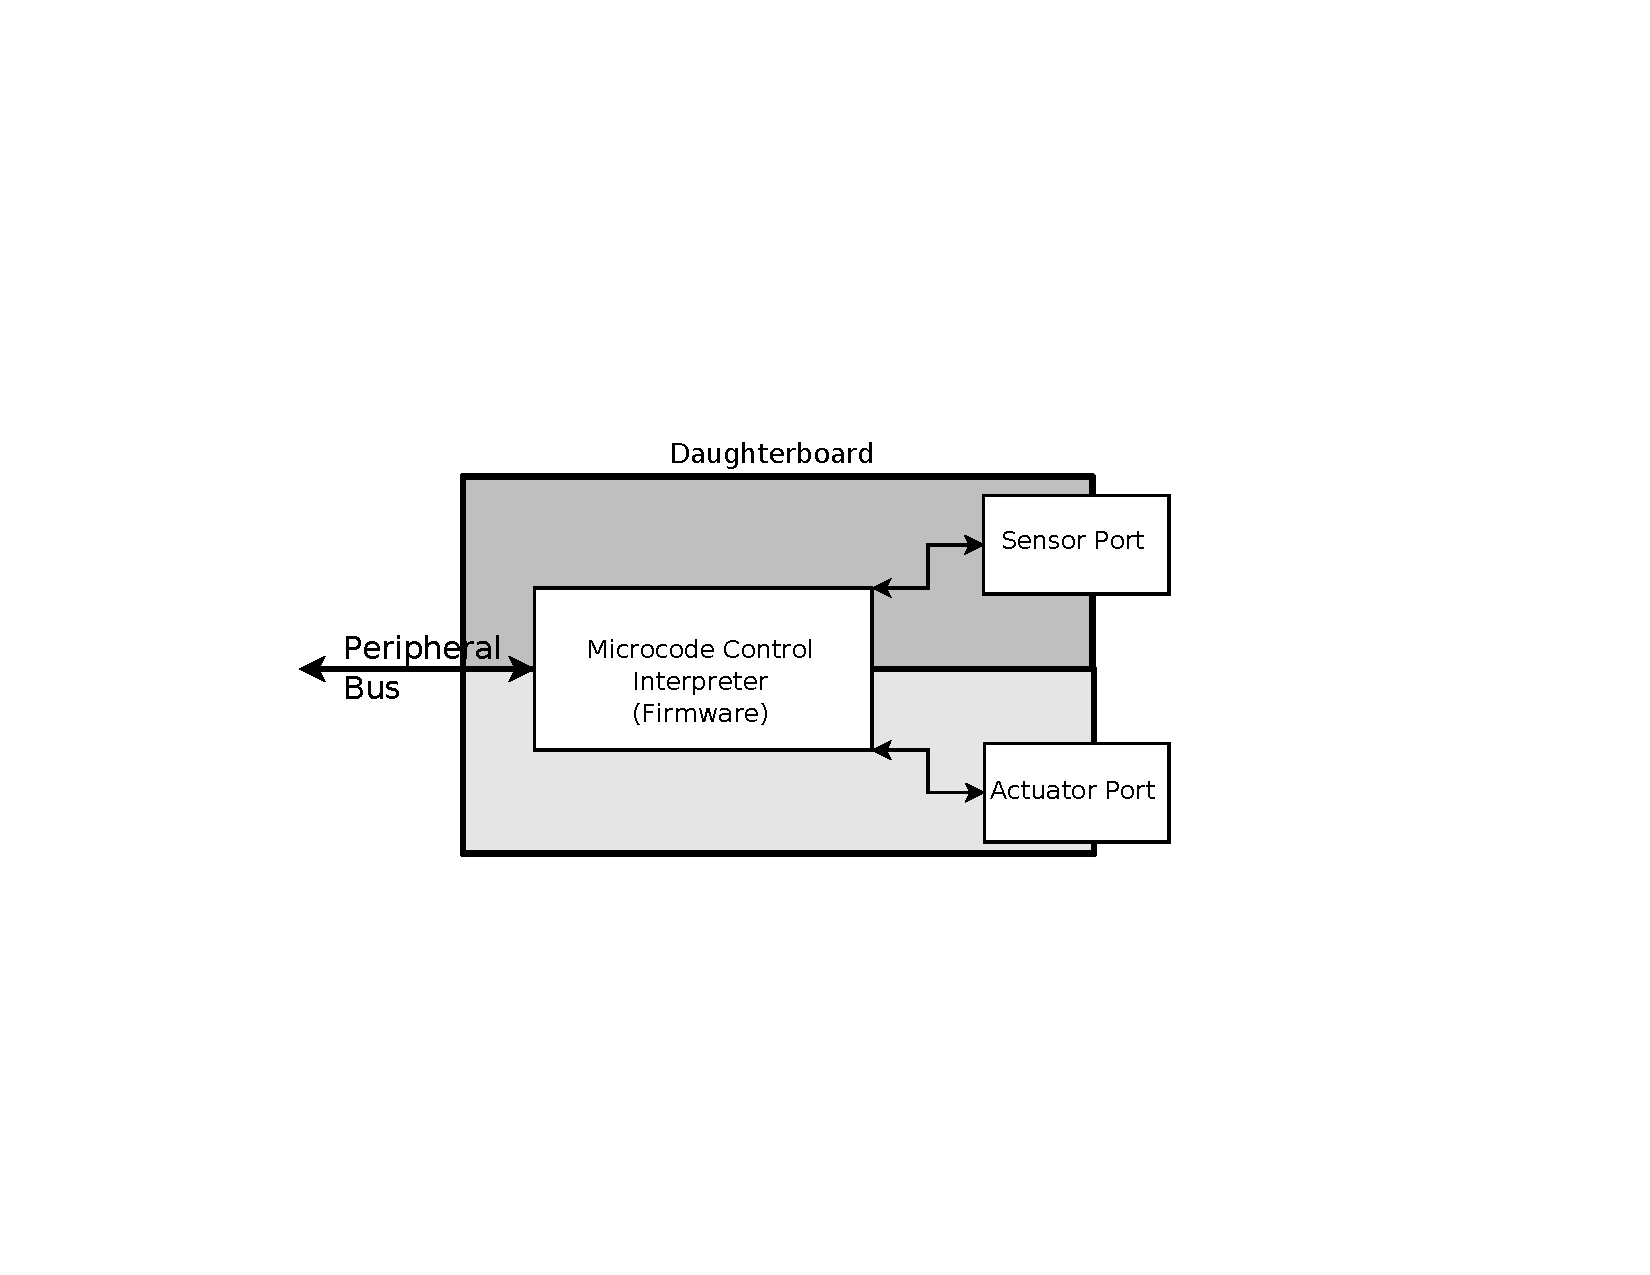
\includegraphics[width=1.0\columnwidth]{Figures/db.pdf}
	    \caption{The daughterboard slave module}
	  \end{center}
	\end{figure}
	
	% subsubsection the_daughterboard (end)
	\subsubsection{Sensor \& Actuator Ports} % (fold)
	\label{ssub:input_&_output_ports}
	All sensors and actuators connect to daughterboards to send and receive data through their respective sensor and actuator ports. Ports are specially designed interfaces that were made to facilitate all types of sensors and actuators. They were built with the most common technological requirements of popular sensors and actuators. The ports are made of up to six(6) pins connected to the daughterboard which should suffice for most operations a sensor or actuator may need to perform.

\begin{figure}[h]
  \begin{center}
    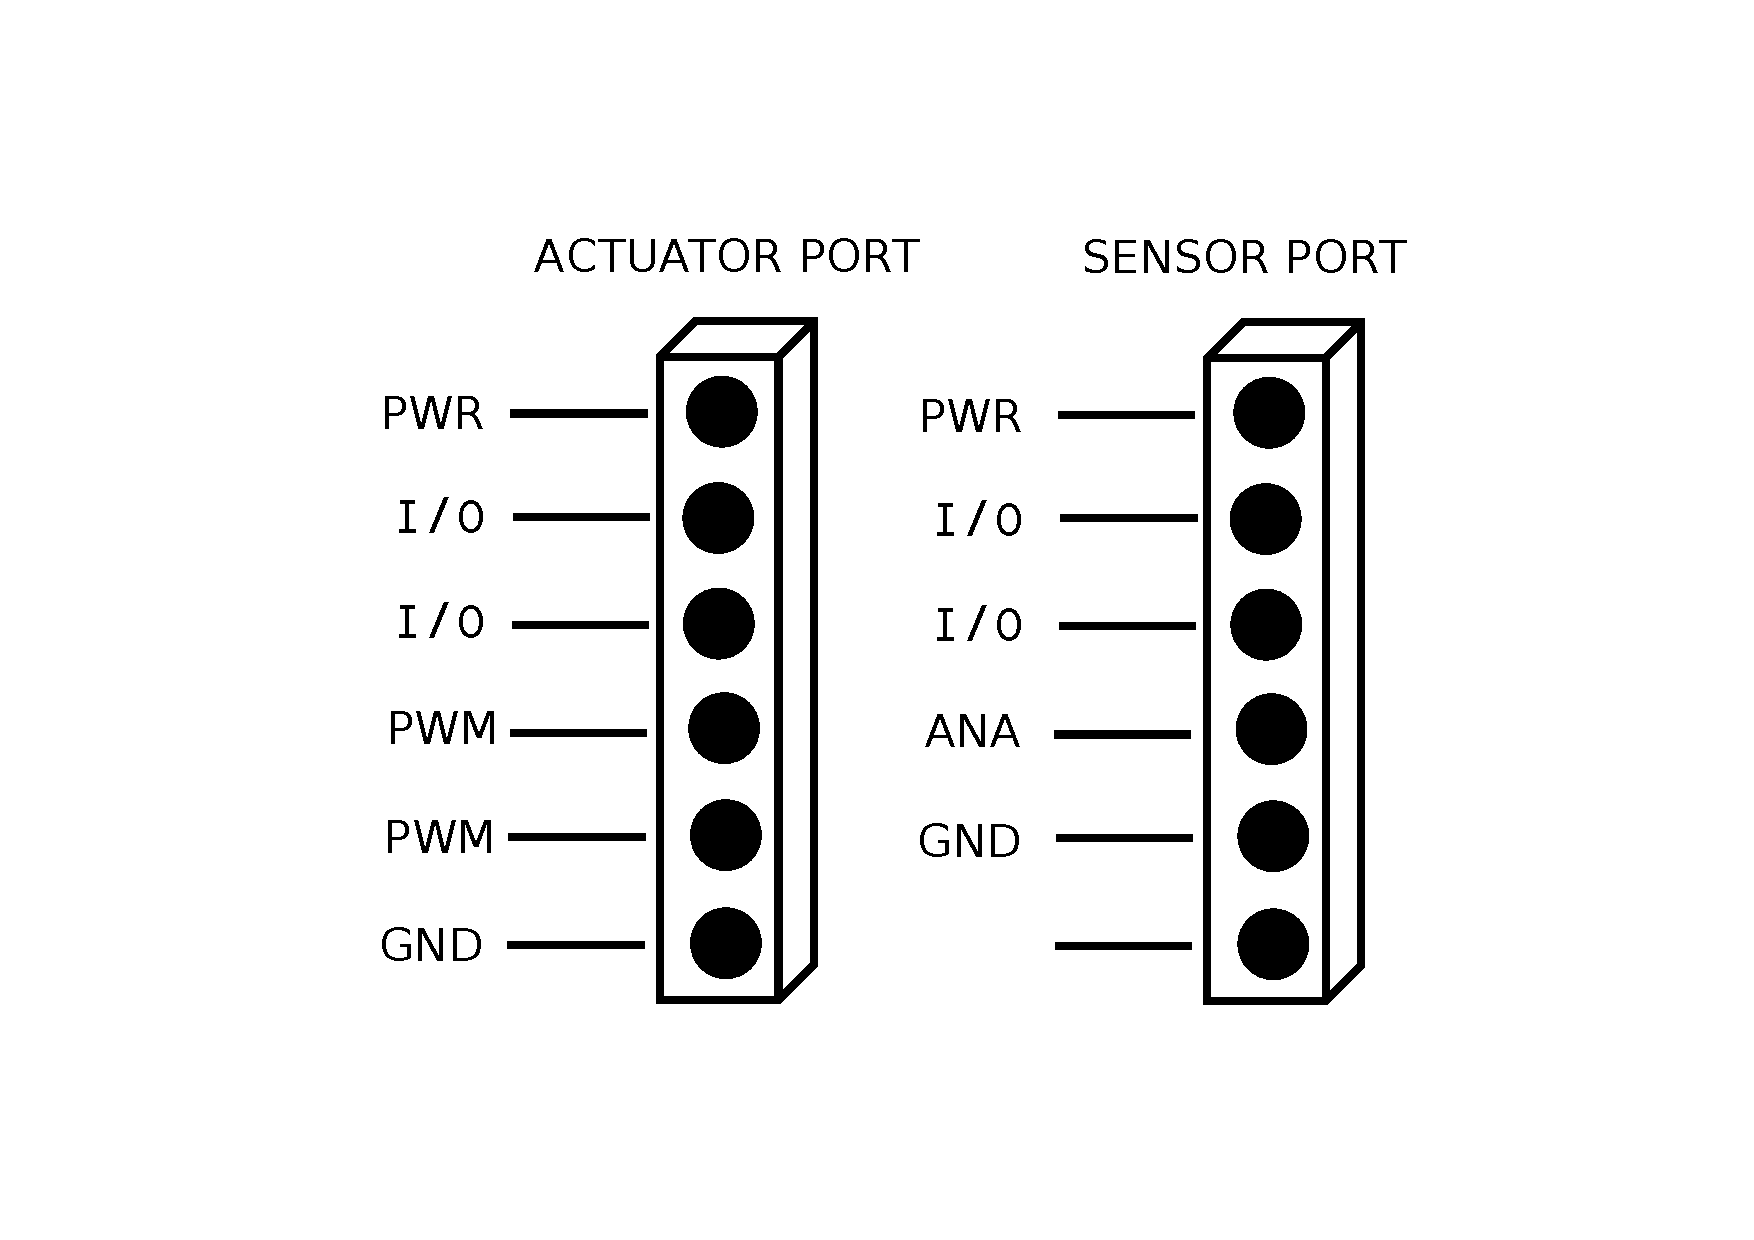
\includegraphics[width=0.5\columnwidth]{Figures/Ports.pdf}
    \caption{The sensor and the actuator ports.}
  \end{center}
\end{figure}

 A sensor port is comprised of five(5) pins: power and ground, an analogue input, and two digital I/O pins. The analogue input pin is able to read voltages from analogue sensors e.g. touch, light and sound sensors. The digital I/O pins can support active and passive digital sensors such as ultrasonic rangefinders,  passive infrared(PIR) sensors and Radio-frequency identification(RFID) sensors. The power and ground pins provide electrically isolated power for the sensors (typically 5 volts, but in principle it could be different from the microcontroller's voltage requirements).

An actuator port is comprised of 6 pins: power and ground, two (2) Pulse Width Modulation (PWM) output pins and two (2) digital I/O pins. The PWM signals allow support for servo motors as well as for adjusting power levels on output devices. The digital I/O pins are able to drive dc motor H-bridges or to be read as digital encoder signals. Like the sensor ports, the power supply for output ports is also electrically isolated from that of the microcontroller. This is particularly necessary when powering motors to prevent damage to the controller and other electronics.

A power bus runs through each daughterboard, connecting all the power pins of its ports. This power bus is meant to supply an alternate power source to the attached sensors and actuators. This alternate power source may or may not be suitable for powering the internal circuitry on the daughterboard, therefore, it is properly isolated.  The power bus terminates as connectors on either side of the board This facilitates daisy chaining the power across the daughterboards, or if necessary, providing separate power supplies for individual modules. Indeed, the scalability of the \xten architecture is more likely to be limited primarily by power considerations than by controlling software or the number of available ports.
	% subsubsection input_&_output_ports (end)
% subsection the_hardware_architecture (end)
\newpage

\subsection{The Software Architecture} % (fold)
\label{sub:the_software_architecture}
The \xten hardware is managed by software distributed across both the motherboard and daughterboard that is responsible for the efficient operation of the system. The software managing the architecture can be classified into four categories: firmware, middleware, device libraries and application software. The application software, libraries and middleware reside on the motherboard while the daughterboards hosts the firmware. Unlike the hardware architecture, we will be describing the software with direct relation to our particular implementation on the Arduino embedded system platform.
	

	\subsubsection{The Motherboard Library} % (fold)
	\label{ssub:the_motherboard_library}

	
	The motherboard robotics library is a toolchain of functions written specifically for robotics applications. We defined and developed an extensible library of useful robotics operations for common devices and general sensors and actuators. They can be composed to control the behavior of a robot. Our particular implementation made use of the Arduino platform which supports the addition of third-party libraries. This allows for robotics developers to take advantage of the usability of the Arduino development platform while capitalizing on the usefulness of a robotics-specific set of operations implemented in the library.
The library was designed not only to provide common robotics functionality to its users but to also make programming large robots with many sensors and actuators less of a hassle especially when taking advantage of the scalability and modularity of the entire platform.

	\begin{figure}[h]
	  \begin{center}
	    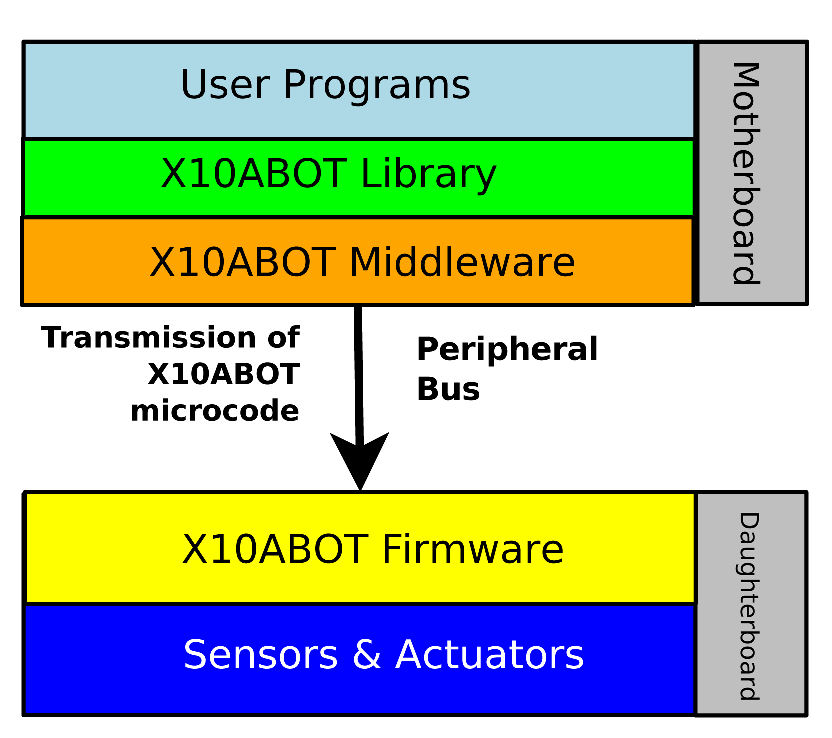
\includegraphics[width=0.7\columnwidth]{Figures/system.pdf}
	    \caption{The \xten software architecture}
	  \end{center}
	\end{figure}
	
	


	% subsubsection the_motherboard_library (end)
	\subsubsection{Application Software} % (fold)
	\label{ssub:application_software}
	Code written by users that takes advantage of the features of the \xten architecture to complete a particular task is considered to be application software. The main purpose for creating a robotics framework is to allow the end user to have a gratifying experience when developing software for their robotics project. We wanted to provide the user with the tools that will allow them to build more interesting robotics projects, without the usual limitations of scale or complexity that may follow. 
	
	We used Arduino's Processing language as our choice for the implementation of the framework. It is know to be very easy to learn and use and also has a supporting IDE that allows the user to get up and started in a short period of time. 
	Applications will be written in a C-like syntax and compiled to run on an Arduino board. This is a familiar interface for many roboticists because Arduino is a very common robotics development platform.
	% subsubsection application_software (end)
	
	\subsubsection{The Daughterboard Firmware} % (fold)
	\label{ssub:the_daughterboard_firmware}
	The daughterboard firmware allows it to provide a standard interface from all daughterboards to their motherboard. All instructions to control or access sensors and actuators are communicated to it via the peripheral bus. These instructions are written as microcode abstractions of the hardware and need to be translated to actual assertions on the devices. Each abstracted command in the motherboard's \xten Library is translated into one or more microcode hardware instructions. Microcode instructions are carried out sequentially by the daughterboards to manipulate the physical hardware components that are attached to their ports. The microcode instructions define a universal set of hardware operations. When these are logically put together, they can control virtually any typical robotics sensor or actuator.
		The microcode instructions specified for daughterboards, provide different means of interacting with each port (see Table~\ref{tab:microcode}).
	The firmware on the daughterboards will interpret these instructions and execute hardware procedures. These instructions are asserted to the standard sensor and actuator ports which are composed of pins, each with their specific purpose. Sensors and actuators are connected to their respective ports and respond to the assertions placed upon them by the daughterboard.
	
	\begin{table}[h] 
	  \scriptsize {%
	    \newcommand{\mc}[3]{\multicolumn{#1}{#2}{#3}}
	    \begin{center}
	      \begin{tabular}{|lll|}\hline %\mc{3}{|c|}{\textbf{}} \\\hline
	        \mc{1}{|c|}{\textbf{Category}} & \mc{1}{c|}{\textbf{Input/Output}} &
	        \mc{1}{c|}{\textbf{Data}}
	        \\\hline \mc{1}{|l|}{Digital I/O } & \mc{1}{l|}{Read/Write} & HIGH/LOW
	        \\\hline \mc{1}{|l|}{Analogue} & \mc{1}{l|}{Read} & n/a
	        \\\hline \mc{1}{|l|}{PWM} & \mc{1}{l|}{Write} & Frequency and Duty Cycle
	        \\\hline \mc{1}{|l|}{I$^{2}$C} &
	        \mc{1}{l|}{Read/Write} & Serial Data\\\hline \mc{1}{|l|}{RS-232} &
	        \mc{1}{l|}{Read/Write} & Serial Data
	        \\\hline \mc{1}{|l|}{Watch} & \mc{1}{l|}{Rising/Falling Edge,
	        } & Threshold Value
	        \\ \mc{1}{|l|}{~} & \mc{1}{l|}{Threshold} & ~
	        \\\hline \end{tabular}
	    \end{center} }
	  \caption{The complete set of hardware operations supported by the
	    microcode interface to the daughterboards.}
	  \label{tab:microcode}
	\end{table}
	\normalsize
	
 The microcode instructions are a universal set of hardware operations restricted to the types of sensors and actuators that are in common use (e.g. analogue, digital, serial, PWM). If a future sensor or actuator should use an incompatible operation, then a firmware upgrade which would include the new microcode instructions would have to be developed in order to interface with it (assuming that it could be made to be hardware compatible with the port). The microcode instructions are made to be very generic, ensuring compatibility with as many sensors and actuators as we could find at the time of design.

	
	The motherboard implements a number of functions that allow the libraries to utilize microcode instruction in the development of device libraries. These instructions are passed to the daugterboard were they are interpreted and executed. Code example ~\ref{code:micro} shows a few of the microcode instructions used in the \xten library and their related parameters.
	
	\begin{listing}[H]
		\footnotesize
		\begin{minted}[bgcolor=bg,frame=lines,framesep=2mm,label={Microcode Functions }]{c}
	

/**
 * @param  byte  state  The state of the digital pin, HIGH(2), LOW(1), INPUT(0)
 * @param  byte  db_address The daughterboard address , 0 for motherboard 
 * @param  byte  port_number The daughter board's port number connected to the device
 * @param  byte  pin_select Choose which of the I/O pins on the port to use A(0) or B(1)
 * @param  byte  pwm_select Choose which of the PWM pins on the port to use A(0) or B(1)
 * @param  byte  duty_cycle Specify the duty cycle as a number between 0 and 255
*/
  void digitalOut(byte state, byte db_address, byte port_number, byte pin_select);
  byte digitalIn(byte db_address, byte port_number, byte operation);
  void pwm(byte pwm_select, byte db_address, byte port_number, byte duty_cycle);
  int analog(byte db_address, byte port_number);
	
		\end{minted}
		\caption{Example of the \xten microcode instructions used in the Library.} \label{code:micro}
	\end{listing}

	For every event on the daughterboard that is to be triggered, a microcode instruction is sent from the motherboard. The format of the instructions are as follows: The first four bits of the first byte define the instructions to be executed and the next four bits define the specific operation for that instruction. The third byte specifies the daughterboard address and the fourth byte has seven bits for the port number and one bit for the pin selection. Each transmitted instruction has a a sequence number that that is assigned to each microcode instruction in the sequence that it is executed. Some instructions require additional data to complete its operations. The microcode format provides a sequence of data bytes that can be of arbitrary size, it is used in operations where a lot of data maybe transmitted e.g RS-232. \cite{tab:mc-structure} shows the structure of a typical microcode instruction.
	\begin{table}[h] \scriptsize {%
		\label{tab:mc-structure}
	    \newcommand{\mc}[3]{\multicolumn{#1}{#2}{#3}} 
	    \begin{center}
	      \begin{tabular}{|lll|}\hline %\mc{3}{|c|}{\textbf{}} \\\hline
	        \mc{1}{|l|}{Byte 1:} & \mc{1}{l|}{1111XXXX} & \mc{1}{l|}{FUNCTION BYTE}
	        \\\hline \mc{1}{|l|}{Byte 1:} & \mc{1}{l|}{XXXX1111} & OPERAND BYTE
	        \\\hline \mc{1}{|l|}{Byte 2:} & \mc{1}{l|}{11111111} & D.B. SELECTION
	        \\\hline \mc{1}{|l|}{Byte 3:} & \mc{1}{l|}{1111111X} & PORT SELECTION
			 \\\hline \mc{1}{|l|}{Byte 3:} & \mc{1}{l|}{XXXXXXX1} & PIN SELECTION
			 \\\hline \mc{1}{|l|}{Byte 4:} & \mc{1}{l|}{XXXXXXX1} & FUNCTION SEQUENCE NUMBER
	        \\\hline \mc{1}{|l|}{Byte 4|+n} & \mc{1}{l|}{11111111 } & DATA
	        BYTES; n\texttt{>} 0
	        \\\hline \end{tabular} method named on
	    \end{center} }
	  \caption{Byte layout for transmitted microcode} 
	  
	\end{table}
	\normalsize
	
	Code example~\ref{code:instr} shows how microcode instructions are used to compose a particular robotics instruction in the \xten architecture. Here the method named \textbf{``on''} is defined for the Actuator class. The \textbf{power} paramenter is passed as an argument to the function. For negative and positive values of \textbf{power}, separate actions are taken. the same microcode operations are executed but with different parameters.
	\begin{listing}[H]
		\footnotesize
		\label{code:instr}
		\begin{minted}[bgcolor=bg,frame=lines,framesep=2mm,label={Robot Instructions}]{c}
void Actuator::on(byte power){
  if (power>0)
  {
    actuator.pwm(A, _db, _port, 255*power/100);
    actuator.digitalOut(HI,_db,_port,A);
    actuator.digitalOut(LO,_db,_port,B);
  }
  else{
    actuator.pwm(A, _db, _port, 255*abs(power)/100);
    actuator.digitalOut(LO,_db,_port,A);
    actuator.digitalOut(HI,_db,_port,B);
  }
}
	
	
		\end{minted}
		\caption{Example of the a robotic instruction which is comprised of microcode operations.} 
	\end{listing}
	
	
	The purpose of the daughterboard is to interpret these high-level instructions from the motherboard and execute them on the respective sensor or actuator irrespective of the hardware specifics of the daughterboard. This ensures that high level language instructions sent from the motherboard remains platform independent.
	
	
	% subsubsection the_daughterboard_firmware (end)
	
	\subsubsection{Middleware} % (fold)
	\label{ssub:middleware}
	Bakken et al. \cite{bakken2001middleware} defined middleware as follows: ``a class of software technologies designed to help manage the complexity and heterogeneity inherent in distributed systems. It is defined as a layer of software above the operating system but below the application program that provides a common programming abstraction across a distributed system.'' The portion of the \xten software architecture that performs the role of middleware does so by providing the motherboard with a level of abstraction and seamless communication with the daughterboards. The middleware handles communication between devices without exposing the details of the protocol or its requirements and the details of the systems hardware on either end. In fact the middleware is used to determine what type of communication medium and protocol is appropriate and creates a standard platform independent interface for interaction. In other words, The middleware just simply presents a standard interface that communicates data and instructions between both the motherboard and daughterboard.
	In a review of popular robotics middleware, Kramer \cite{Kramer2006} defines cites some major advantages which are applicable to the \xten architecture. He states that it aids in software modularity, which is an intentional design objective. The middleware allows for pluggable libraries at the motherboard level which are ignorant of the actual hardware implementations. This accomplishes the platform independence, and portability that Kramer found to be a common attribute of most robotics middleware.
	
	The aspect of the \xten architecture that transports the microcode from the libraries of the motherboard to the interpreter of the daughterboard is considered to be our middleware. Each microcode instruction formats the byte string as described in Table ~\ref{tab:mc-structure}. The microcode then performs one or more of a series of dispatch and request events between the motherboard and the daughterboard. The daughterboard also initiates data transfers as well for certain special cases. All these operations are managed by the middleware. 
\begin{listing}[H]
\footnotesize
\label{code:instr}
{\fontsize{8}{6}\selectfont
\begin{minted}[bgcolor=bg,frame=lines,framesep=2mm,label={Robot Instructions}]{c}

void X10ABOT_MB::digitalOut(byte state, byte db_address, byte port_number, byte pin_select){
  byte microcode[] = {FN_IO+state,db_address,((port_number-1)<<1)+pin_select,incr_instr_seq()};
  dispatch(microcode, sizeof(microcode));

}

byte X10ABOT_MB::digitalIn(byte db_address, byte port_number, byte pin_select){
  byte seq_num = incr_instr_seq();
  byte microcode[] = {FN_IO+IN,db_address,((port_number-1)<<1)+pin_select,seq_num};
  dispatch(microcode, sizeof(microcode));
  delay(50);
  return requestHandler(microcode, 2,seq_num);
}

void X10ABOT_MB::pwm(byte pwm_select, byte db_address, byte port_number, byte duty_cycle){
  byte microcode[] = {FN_PWM,db_address,((port_number-1)<<1)+pwm_select,incr_instr_seq(),duty_cycle};
  dispatch(microcode, sizeof(microcode));
}

\end{minted}
}
\caption{Example of the a robotic instruction which is comprised of micro-code operations.} 
\end{listing}	

The dispatch and request events are used to
	% subsubsection middleware (end)
	
	\subsubsection{Extending the Library} % (fold)
	\label{ssub:extending_the_library}
	
	To allow for easy extensibility and to support new hardware, the X10ABOT software architecture was designed to allow user extensible libraries. A library defines a set of microcode instructions used to control a hardware device.
	
	New types of sensors and actuators can be supported by adding them as a device library on the the \xten motherboard. Creating a new device specification can be done without the need to understand any low level device specific coding, since all the configurations are abstracted for easier programming. Extensibility is therefore achieved through high-level abstraction of low level hardware components.
	The \textbf{X10} in \xten which stands for extensibility, is one of the key design goals for the architecture. Extensibility defines the ability of the platform to support a vast variety of sensors and actuators with the inherent ability to support new or previously unsupported peripherals. This ability is a significant part of the core framework design. Both the hardware and software allow for inclusion for new and cutting edge technologies by utilizing the simple idea of composition of low level microcode instructions. It can be shown that many seemingly complex protocols or devices operate using only a few simple fundamental electronic operations defined by our microcode instructions\cite{CITE OR SHOW EXAMPLES}. By creating a set of instructions that utilize these fundamental operations, any composite methods can be formed to complete most electronic tasks. For example: to operate a servo motor, this requires a variation in a pulse width modulated signal, a switch can be a simple digital I/O connection, and a light intensity sensor just simply uses an analogue to digital input. 
	The \xten system architecture was designed to facilitate device libraries which operate in a similar sense as hardware drivers for computer peripherals. A driver typically communicates with the device through a communications subsystem to which the hardware connects.	
	% subsubsection extending_the_library (end)
	
	\subsubsection{Multitasking} % (fold)
	\label{ssub:multitasking}
	
	Another major aspect of the software system is its ability to execute simultaneous tasks. This was provided by the LEGO\textregistered Mindstorms\textregistered NXT platform and implemented in the X10ABOT robotics platform using the FreeRTOS real time scheduler. FreeRTOS is a tried and tested open source system which offers a very fast and efficient means of handling multiple tasks and timing operations.
	% subsubsection multitasking (end)
	
	\subsubsection{The X10ABOT LEGO VM} % (fold)
	\label{ssub:the_x10abot_lego_vm}
	There has been significant work toward the creation of a LEGO\textregistered Mindstorms\textregistered NXT virtual machine which will operate on top on the X10ABOT Library. User program code in the form of bytecode will be interpreted and executed with equivalent library commands. Many of the limitations in the hardware of the NXT are not enforced in its bytecode, therefore it may have the ability to utilize the extra sensors and actuator ports provided by the X10ABOT Library.
	% subsubsection the_x10abot_lego_vm (end)
	
% subsection the_software_architecture (end)

% section the_architecture (end)

\section{The Arduino Implementation} % (fold)
\label{sec:the_arduino_implementation}
\xten is a robotics architecture that is indifferent to any particular hardware system. We endeavored to create an architecture that had very few hardware specific restrictions that would force the developer to chose one hardware platform over another. We also tried to create an architecture that was capable of running on systems as simple as 8-bit micro-controllers. What we found was that the majority of hobbyist robotics and robots used in school competitions tended to use 8-bit microcontrollers. However, many of the major notable robotics architectures were built on top of a full featured 32 or 64-bit processing systems\cite{Elkady2012}. The architecture should however be able to scale up to a full scale 32 or 64-bit computer. This will allow for more complex programs to be written with more processor and hardware intensive operations. The most basic requirements for any implementation of the \xten architecture is a microprocessor which has the ability to perform digital and analogue input and output. In this case, one controller will operate as both motherboard and daughterboard. In order to support external daughterboards, each microcontroller must have support for the \iic protocol in addition to the minimum requirements listed above.

The Arduino embedded system framework is a very active project, and it is notable for keeping at the cutting edge of embedded development. The framework is platform independent and currently deployed on a variety of processors including Atmel's AVR 8-bit and 32-bit ARM processors. There are even a few other companies including Microchip who have adopted the Arduino framework for their 32-bit processors as well\cite{Development2012}. 
The \xten software was written with the Processing language supported by Arduino which is a derivative of C++. This allowed us to take advantage of many of C++'s high level language features including class hierarchy which is the basis of how development for the motherboard libraries are done. Arduino also comes with a cross platform IDE that allows development on all the major operating systems.

The Arduino platform provides very inexpensive hardware that can be used for both motherboard and daughterboard. They were designed for physical add-ons called shields which are convenient connection boards that can host auxiliary circuitry like port headers, external power and H-bridges.

% section the_arduino_implementation (end)

 % \chapter{Design and Implementation}
\chapter{Results} 
\label{chap:results}
%\begin{enumerate}
%\item all data
%\item analysis done
%\item discussions
%\item comparisons
%\end{enumerate}
This section seeks to demonstrate the steps taken in the data gathering process, critical data analysis and validation of the effectiveness of models developed. We start by looking at fluid flows in the heart of the UWICSS and extracting parameters for models in Section~\ref{sec:windkessel_data}.  We can then demonstrate the effectiveness of the windkessel/lumped parameter model in predicting the behaviour of the aorta.  In validating the hydraulic system for the UWICSS, we also examine the effect of the mechanical delays for the valves and pumps.  These mechanical delays are a hindrance to the precise manipulation of fluid pressure and a direct limitation on the maximum frequency achievable by the controller.

This section also discusses the results drawn from the implementation of designs detailed in Chapter~\ref{chap:design}.  There are some important conclusions that can be made about the overall system and the numerical controller:
\begin{itemize}
\item The system based controller described in Chapter~\ref{chap:design}, is capable of achieving a maximum pulse frequency of 0.6 pulse per second.
\item The parameters of the two element windkessel model used in the system, can be successfully derived using known principles.
\item The current firmware architecture can be used to implement the numerical controller discussed in Section~\ref{sec:controller_design} of this thesis.
\item In order to achieve precise manipulation of fluid pressure between 0.4 pulse per second and a maximum of 6 pulses per second, faster actuations are required.
\item Comparison of the performance results between the system with mechanical delays and that of the system without these delays, shows the reduction in the performance of the controller.
\end{itemize}

\section{Results from Calibration of Sensors}

% chapter 3 the \texttt{x10abot_architecture_design_and_implementation (end)
%\chapter{Findings and Results} % (fold)
%\label{cha:findings_and_results}



\begin{figure}
  \begin{center}
    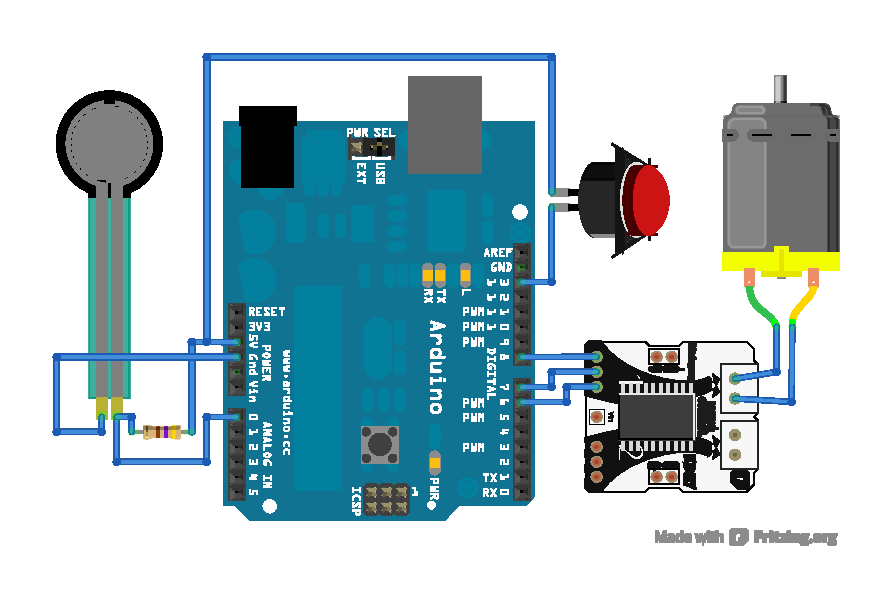
\includegraphics[width=1.0\columnwidth]{Figures/simple-example.pdf}
    \caption{The components of a simple singleboard \xten Example}
  \end{center}
\end{figure}

The following chapter demonstrates how the \xten architecture achieves its objectives through the hardware and software platform. We will demonstrate how the framework can be applied in a practical manner and we will explain the outcomes.

 We will demonstrate the framework in action by showing excerpts of sample programs for a simple mobile robot with a number of sensors and actuators distributed across one or more daughterboards.
%[mathescape,linenos, gobble=2,]


Code example~\ref{code:example} is a typical setup for a very simple mobile robot. All the sensors are on one daughterboard - in the case of our implementation, the ``internal'' daughterboard which is hosted on the same board as the motherboard. This robot has one actuator (a DC motor connected to an external H-bridge), a force sensor and a pushbutton sensor.


%\begin{multicols}{2}
	\begin{listing}
		\footnotesize
		\begin{minted}[bgcolor=bg,frame=lines,framesep=2mm,label={\xten Sample code}]{c}

/**
* Import the necessary libraries for the motherboard, 
* daughterboard and the peripheral bus
**/
#include <Wire.h>  
#include <X10ABOT_MB.h>
#include <X10ABOT_DB.h> //Included to support the internal daughterboard #0

//Declare and initialize motor on daughterboard #0, actuator port #1
Actuator motor1(0,1);
//Declare  and initialize force sensor on daughterboard #0, sensor port #1
Sensor force1(0,1);
//Declare  and initialize force sensor on daughterboard #0, sensor port #2
Sensor pushbutton(0,1,B);

void setup(){}

void loop(){
//Continuously check the sensors for a reading
if(pushbutton.readDigital() || (force1.readAnalogue()>100)){
  motor1.on(100); //Turn motor1 on at full power (100%) 
  }else{
  motor1.off();  //Turn motor1 off
  }
}	 

		\end{minted}
		\caption{Example of the \xten architecture on a simple robot.} \label{code:example}
	\end{listing}
%	\vfill
%	\columnbreak



Code example~\ref{code:example} is a simple program that drives the motor in the forward(positive) direction at full speed if either the touch sensor records an input or if there is a force on the force sensor about a certain threshold, otherwise it will shut off the motors.

%\end{multicols}
In this instance, there are two types of devices that are declared, \textbf{Sensors} and \textbf{Actuators}. These represent the parent classes of all sensors and actuators respectively in the \xten architecture. All other sensor and actuator sub-types inherit from these two classes of devices, overriding where necessary.

It should be noted that it was necessary to include the library for both the motherboard and the daugterboard because the daughterboard and motherboard shares the same Arduino board. Daughterboard address \#0 is reserved for the internal or resident daugterboard on the same physical Arduino platform.

	\section{Modularity} % (fold)
	\label{sec:modularity}
% section modularity (end)
%Adding extra capability can be easily and seamlessly done using the \xten architecture. An extra daughterboard can represent a complete subsystem using sensors and actuators. A reasonable %example could be a simple robotic arm used to fetch items based on readings from one or more attached sensors. The \xten architecture allows for these new devices on separates %daughterboard to be attached via the perpheral bus. These modules can be just as easily added in software. Each daughterboard containing sensors and actuators can be declared with a unique %address similar to the existing modules. Instructions can then be added for its application.
 In the code example~\ref{code:modularity}, we see how an extra sensor and an actuator was added for an extra functionality. 

\begin{figure}[h!]
  \begin{center}
    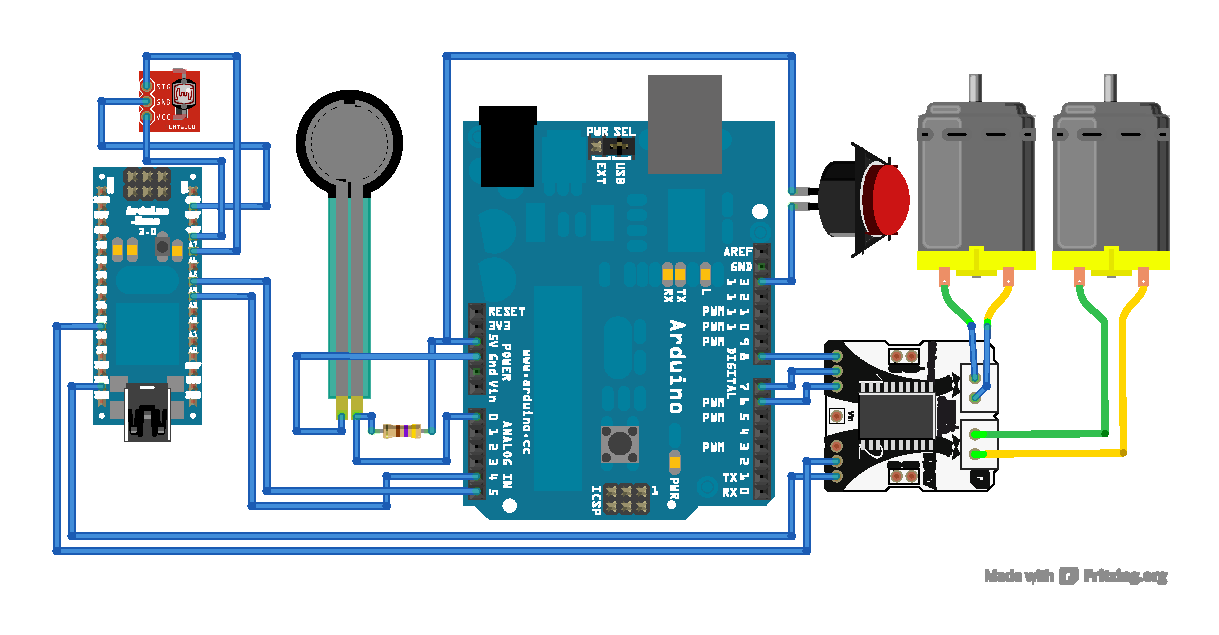
\includegraphics[width=1.0\columnwidth]{Figures/modular-example.pdf}
    \caption{The components of a Modular singleboard \xten Example}
  \end{center}
\end{figure}

\begin{listing}
		\footnotesize
		\caption{Example of modularity in action.} \label{code:modularity}
		\begin{minted}[bgcolor=bg,frame=lines,framesep=2mm,label={Modularity in Code}]{c}
/**
* Import the necessary libraries for the motherboard, 
* daughterboard and the peripheral bus
**/
#include <Wire.h>  
#include <X10ABOT_MB.h>
#include <X10ABOT_DB.h> //Included to support the internal daughterboard #0

//Declare motor on daughterboard #0, actuator port #1
Actuator motor1(0,1);
//Declare force sensor on daughterboard #0, sensor port #1
Sensor force1(0,1);
//Declare force sensor on daughterboard #0, sensor port #2
Sensor pushbutton(0,1,B);
//Declare motor on daughterboard #9, actuator port #1
Actuator motor2(9,1);
//Declare force sensor on daughterboard #9, sensor port #1
Sensor lightSensor(9,5);

void setup(){}
void loop(){
//Continuously check the sensors for a reading
if(pushbutton.readDigital || force1.readAnalogue()){
  motor1.on(100); //Turn motor1 on at full power (100%) 
}else{
  motor1.off();  //Turn motor1 off
  }
//Added extra functionality with a new sensor and a new actuator on daughterboard #9
//while motor1 is running and light is on the sensor, activate motor2
if (motor1.isOn() && lightSensor.readAnalogue())
  {motor2.on(-50); //Turn motor2 on at 50% in the reverse direction
  }else{
  motor2.off();  //Turn motor2 off
  }
}	 
	\end{minted}
		
\end{listing}
In this particular example (code~\ref{code:modularity}), even though \emph{motor1} and \emph{lightSensor}, two additional, independent devices were added to the system, it did not affect the existing code but fit seamlessly in the development process. Separate code was added to carry out its operation which never needed to interact with the exisiting system. There needed to be no special acccomodation for the new module in the existing system. There also was no hardware modification made to the existing setup even with the fact that an extra physical component, another daughterboard, was added to the system.
All these features are an indication of a truly modular architecture. As previously defined, we included an entire subsystem without modifying the existing components. The modules can be removed just as easy as they were installed. The level of expertise required to modify this system is also relatively minimal due to its design.


% chapter findings_and_results (end)
\section{Extensibility and Abstraction} % (fold)
\label{sec:extensibility_abstraction}
We demonstrate the \xten architecture's ability to support new and varied types of sensors and actuators. This is accomplished with no knowledge of the low-level details of the hardware.
In the following example, we will define a simple, yet complete library that reads and interprets the data from a thermistor temperature sensor. The temperature value will be returned in fahrenheit units. This code was sourced from the Arduino Playground \parencite{therm} as a simple example to acquire thermistor temperature readings. We made a simple modification that allowed the same code to be applicable to the \xten architecture.
\begin{listing}
		\footnotesize
		\caption{Example: A complete library for a thermistor temperature sensor.} \label{code:therm}
		\begin{minted}[bgcolor=bg,frame=lines,framesep=2mm,label={Thermistor Library}]{c}
#include <Sensor.h>
#include <math.h>

double readThermister() {
 int RawADC = analog(_db,_port);
 double Temp;
 Temp = log(((10240000/RawADC) - 10000));
 Temp = 1 / (0.001129148 + (0.000234125 + (0.0000000876741 * Temp * Temp ))* Temp );
 Temp = Temp - 273.15;            // Convert Kelvin to Celcius
 Temp = (Temp * 9.0)/ 5.0 + 32.0; // Convert Celcius to Fahrenheit
 return Temp;
}
	\end{minted}
		
\end{listing}

The library in code example \ref{code:therm} above is an almost exact replica of the fragment of code extracted from the Arduino library. The code accesses the analogue pin to read the sensor. The \xten framework possesses special functions that access hardware components. For this particular case, the \textbf{analog(\_db,\_port)} function was invoked. This is a method used to abstract the analog pin so it becomes hardware independent. The analogue pin here is perceived as a virtual entity that belongs on a daughterboard \textbf{\_db} on a particular port \textbf{\_port}. The result is then returned to the calling function, presenting the temperature value to the user in Fahrenheit.

This thermistor library can then be easily utilized by the user as follows:

The code in code example~\ref{code:thermcode} presents a temperature monitoring system that watches the temperature that it receives from two thermistors. If the value read from the thermistors goes beyond particular thresholds for either of them, an alarm is triggered.
\begin{listing}
		\footnotesize
		\caption{Example application of the thermistor temperature sensor library.} \label{code:thermcode}
		\begin{minted}[bgcolor=bg,frame=lines,framesep=2mm,label={Thermistor Example Application}]{c}
#include <Wire.h>  
#include <Thermistor.h>  
#include <X10ABOT_MB.h>

//Declare motor on daughterboard #17, actuator port #1
Thermistor temp1(17,1);
//Declare force sensor on daughterboard #108, sensor port #6
Thermistor temp2(108,6);
//Declare digital alarm on daughterboard #10, sensor port #3
Buzzer alarm(10,3,A);

void setup(){}
void loop(){
//Continuously check the sensors to see if temperature within threshold
  if((temp1.readThermister() > 70 )|| temp1.readThermister()<30){
  alarm.on(); //Turn on alarm 
}
	\end{minted}
		
\end{listing}

The library for was included and it became pretty straightforward to manipulate the sensor afterwards.
% section extensibility and abstraction (end)

\section{Scalability} % (fold)
\label{sec:scalability}

% section scalability (end)
The results for the application on modularity are two fold and can be seen clearly to imply scalability. The method of modular additions is scalable to tens of modules as defined by the peripheral bus protocol. We therefore need to benchmark the performance of the architecture implemented on the Arduino platform. This is necessary to evaluate the speed at which instructions are excuted. This can determine how the system will perform when under duress from multiple hardware devices simultaneously. These statistics can then be evaluated to deduce the architecture's suitability for a particular project. The \xten architecture's major limiting factor is the speed of the peripheral bus, however, other hardware specific limitations may come into play. These may include, clock speed and available RAM, all of which may differ, even across Arduino hardware platforms. All tests below were carried out on the Arduino Mega, using the Atmel \texttrademark ATMega1280 microcontroller.

We carried out a few timing tests to evaluate the performance of the \xten framework on the Arduino platform. The test were done using one motherboard and three daughterboards. The typical robotics project may never require as many daughter boards since one Arduino Mega may support up to eight sensor ports and six actuator ports. The smaller Arduino Uno can support up to three sensor ports and two actuator ports. Any combination of one or more of these Arduino boards can be used to implement the \xten architecture.
We did timing tests to measure the latency between the command request and the response. We also recorded the measurable difference when the peripheral bus is congested with a rapid succession of events for all the six daughterboards.

The tables below display the results of our timing experiments, the timing utility on the Arduino has a maximum resolution of 4 micro second intervals.

\begin{table}[h!]
    %\scriptsize {
	%\centering
	\caption{Table showing microcode latency in microseconds($\mu$s) on the on-board daughteroard over 20 consecutive executions.}
	\begin{tabular}{|l|l|l|l|}
	\toprule
 \multicolumn{4}{c}{\textbf{ONBOARD daughterboard}} \\\hline

digitalOut & digitalIn & pwm & analogue \\\hline
40 & 50084 & 60 & 50212\\\hline
40 & 50088 & 60 & 50216 \\\hline
40 & 50084 & 60 & 50212 \\\hline
36 & 50084 & 60 & 50216 \\\hline
40 & 50084 & 56 & 50212 \\\hline
40 & 50084 & 60 & 50212 \\\hline
40 & 50084 & 60 & 50212 \\\hline
40 & 50080 & 60 & 50216 \\\hline
40 & 50084 & 60 & 50216 \\\hline
48 & 50080 & 56 & 50216 \\\hline
40 & 50088 & 56 & 50216 \\\hline
40 & 50084 & 56 & 50216 \\\hline
40 & 50084 & 60 & 50216 \\\hline
36 & 50084 & 60 & 50216 \\\hline
40 & 50080 & 60 & 50220 \\\hline
40 & 50084 & 64 & 50216 \\\hline
40 & 50084 & 56 & 50216 \\\hline
40 & 50080 & 60 & 50224 \\\hline
40 & 50084 & 56 & 50216 \\\hline
\multicolumn{4}{c}{Average Times} \\\hline
40.00 & 50083.58 & 58.95 & 50215.58

%}
\end{tabular}
\end{table}

The latency for output operations was significantly less time than that of input operations. This was expected since there is no waiting period to request the value of the data from the port on the daughterboard for output operations.  

\begin{table}
    %\scriptsize {%
	\centering
	\caption{Table showing microcode latency in microseconds($\mu$s) on the off-board daughteroard over 20 consecutive executions.}
	
	\begin{tabular}{|l|l|l|l|}
	\toprule
 \multicolumn{4}{c}{\textbf{OFFBOARD daughterboard}} \\\hline
digitalOut & digitalIn & pwm & analogue\\\hline
568 & 51320 & 688 & 51328\\\hline
560 & 51320 & 684 & 51320\\\hline
568 & 51324 & 684 & 51324\\\hline
568 & 51324 & 684 & 51328\\\hline
568 & 51332 & 684 & 51324\\\hline
564 & 51324 & 684 & 51332\\\hline
564 & 51324 & 684 & 51328\\\hline
564 & 51320 & 688 & 51324\\\hline
564 & 51320 & 680 & 51332\\\hline
568 & 51324 & 688 & 51324\\\hline
564 & 51324 & 680 & 51324\\\hline
568 & 51324 & 684 & 51324\\\hline
564 & 51320 & 684 & 51328\\\hline
568 & 51328 & 684 & 51324\\\hline
560 & 51320 & 688 & 51328\\\hline
564 & 51320 & 688 & 51328\\\hline
568 & 51324 & 684 & 51332\\\hline
564 & 51320 & 684 & 51324\\\hline
564 & 51320 & 684 & 51324\\\hline
\multicolumn{4}{c}{Average Times} \\\hline
565.26 & 51322.74 & 684.63 & 51326.32

%}
\end{tabular}
\end{table}

We carried out an experiment to determine how the system performed when executing a barrage of instruction and obtained the results lsted in table X below. 
\begin{table}
    %\scriptsize {%
	\centering
	\caption{Table showing microcode latency in microseconds($\mu$s) on the off-board daughteroard for number of instructions executed(no.) and associated time it took to complete over 5050 consecutive executions of digitalOut.}
	
	\begin{tabular}{|l|l||l|l||l|l||l|l||l|l||}
	\toprule
 \multicolumn{10}{c}{\textbf{OFFBOARD daughterboard barrage}} \\\hline


no. & time ($\mu$s)& no. & time ($\mu$s)& no. & time ($\mu$s)& no. & time ($\mu$s)& no. & time ($\mu$s) \\\hline
1 & 568 & 21 & 11840 & 41 & 23120 & 61 & 34380 & 81 & 45648 \\\hline
2 & 1132 & 22 & 12412 & 42 & 23676 & 62 & 34936 & 82 & 46216 \\\hline
3 & 1696 & 23 & 12972 & 43 & 24244 & 63 & 35516 & 83 & 46780 \\\hline
4 & 2268 & 24 & 13524 & 44 & 24796 & 64 & 36080 & 84 & 47352 \\\hline
5 & 2820 & 25 & 14108 & 45 & 25364 & 65 & 36620 & 85 & 47916 \\\hline
6 & 3384 & 26 & 14656 & 46 & 25932 & 66 & 37208 & 86 & 48480 \\\hline
7 & 3948 & 27 & 15228 & 47 & 26484 & 67 & 37772 & 87 & 49044 \\\hline
8 & 4520 & 28 & 15788 & 48 & 27068 & 68 & 38332 & 88 & 49600 \\\hline
9 & 5072 & 29 & 16352 & 49 & 27620 & 69 & 38880 & 89 & 50172 \\\hline
10 & 5636 & 30 & 16908 & 50 & 28188 & 70 & 39456 & 90 & 50736 \\\hline
11 & 6212 & 31 & 17472 & 51 & 28760 & 71 & 40028 & 91 & 51296 \\\hline
12 & 6768 & 32 & 18044 & 52 & 29316 & 72 & 40588 & 92 & 51860 \\\hline
13 & 7332 & 33 & 18600 & 53 & 29872 & 73 & 41156 & 93 & 52420 \\\hline
14 & 7896 & 34 & 19172 & 54 & 30452 & 74 & 41696 & 94 & 52980 \\\hline
15 & 8460 & 35 & 19732 & 55 & 31008 & 75 & 42276 & 95 & 53552 \\\hline
16 & 9020 & 36 & 20300 & 56 & 31552 & 76 & 42844 & 96 & 54112 \\\hline
17 & 9584 & 37 & 20856 & 57 & 32140 & 77 & 43408 & 97 & 54672 \\\hline
18 & 10148 & 38 & 21424 & 58 & 32696 & 78 & 43976 & 98 & 55244 \\\hline
19 & 10708 & 39 & 21988 & 59 & 33248 & 79 & 44536 & 99 & 55804 \\\hline
20 & 11280 & 40 & 22548 & 60 & 33828 & 80 & 45096 & 100 & 56364 \\\hline
\multicolumn{10}{c}{Total time taken: 2847984} \\\hline
\end{tabular}
\end{table}
 The results showed that even at high instruction thoroughput, the time to execute a particular instruction does not vary significantly from its latency as a single instruction.


\section{Economy} % (fold)
\label{sec:economy}

% section economy (end)
 % \chapter{Results and Discussion}
\chapter{Conclusion and Discussion} 
By actualising the architectural design concepts of modularity, scalability and extensibility discussed in Chapter~\ref{cha:background_and_motivation}. We were able to create a platform that effectively accomplished these required objectives. We have also realised that this design framework has created an extensible platform for numerous avenues of future work. There are opportunities to support various programming interfaces, porting \xten to more powerful hardware and support of additional sensor and actuator devices.

\section{Limitations}
The efficiency of the \xten architecture is limited by the speed of its peripheral bus, which in our case is \iic and the power of the processors that implement it.
The limitation details are listed below:
\begin{itemize}
\item Our implementation was done on an 8-bit Arduino processor running at 16MHz with 8KB of SRAM. This inherently limited the kinds of tasks that could have been attempted. This is not an insurmountable obstacle however for most projects within the scope of the target user's applications, this would be adequate. There have also been recent advancement in the Arduino community where there is now available 32-bit Arduinos running at 84Mhz with 96KB of SRAM. Using this hardware could increase the speed of operations on the \xten, possibly positively impacting the data in the results section of this thesis without significantly increasing the overall cost. This would be mostly due to the ability of faster processing of instructions. Porting the existing code base to this platform would require very minor changes since Arduino code is mostly hardware independent across other Arduino compatible products.

\item Communication between motherboard and daughterboard are limited by the speed on the \iic bus which is not only limited by its specification but the clock speed of the host processor. As mentioned previously, better hardware would overcome this limitation. Applications which may require a more powerful system may include ones with significant video processing.
\item Other limitations include the \iic 112 device limit on the peripheral bus, and the limit of 16 sensors and actuators (8 each) per daughterboard. These limits are relatively very high and are more than adequate for applications within the scope of this project.
\item To achieve the goals of modularity, scalability and extensibility, we made a design decision to create specialised input and output ports. These ports are further specialised by having pins dedicated to certain functionalities. This decision limits the number of devices that can be attached per daughterboard to the number of ports that daughterboard supplies. However we compared the number of ports when utilising a motherboard and a daughterboard from an Arduino (4 sensor ports, 6 actuator ports) to the number provided by a popular kit like the LEGO Mindstorms NXT (4 sensor ports, 3 actuator ports) and based on a cost per port comparison, ~\$60 and ~\$260 US dollars respectively, we were in a much better position. Then current implementation of the \xten framework may not be as feature complete as the LEGO Mindstorms NXT but for basic sensors and actuators, it provides a less expensive way to utilize more.
\end{itemize}

\section{Achievements}
The following are a list of the main objectives that were accomplished:
\begin{itemize}
\item \textbf{Designed modular, distributed hardware framework:} We are now able to easily add or remove hardware and software modules in and out out of the system.
\item \textbf{Engineered a model that can support almost 900 sensors and 900 actuators:}Using the theoretic capabilities of the \iic peripheral bus, we are able to support up to 112 daughterboards supporting 8 sensor and 8 actuators each.
\item \textbf{Created an extensible software framework that can support the addition of many types of sensors \& actuators:} Taking advantage of the abstraction of ports and pins accomplished in the framework design, we were able to create a platform for supporting the creation of libraries that support new sensors and actuators.
\item \textbf{Created a flexible system that allows easy interoperability with distinct hardware architectures:} The \xten was designed with a middle-ware type software layer that allows the system to communicate with hardware platforms that are very different from each other, providing that both are using the standard protocol.
\item \textbf{Kept the cost low by using the Arduino as the main hardware component:} The system was designed to be implemented on very inexpensive hardware such as Arduino based devices. It can scale to support a large number of these inexpensive devices.
\item \textbf{Successfully tested the framework with both digital and analog sensors and actuators for latency:}
We benchmarked the system to determine its suitability for robotics applications which student's and hobbyists may pursue. We found the performance to be acceptable and where more power is required, more powerful hardware can be acquired.
\end{itemize}



We can therefore conclude that the \xten architecture provides a suitable platform that will enable efficient robotics development for our target audience of students and hobbyists. It will accomplish this by providing a model that can scale to a large number of sensors and actuators. This was made possible by utilising a distributed modular framework of daughterboards that can be attached whenever needed. We performed tests to measure the latency of I/O instructions between the peripheral devices and the motherboard. We found it to be in an acceptable range that was tolerable for most robotics applications within the scope of 8-bit microprocessors. This delay time would also see improvements if the processor and communication speeds were increased. The performance of the system is dependent upon the hardware that implements it.

\section{Future Work}
In order to facilitate processor intensive operations, the architecture would have to be ported to a more powerful hardware platform. At the time of writing, there was a recent release of an Arduino based on the 32-bit, 84Mhz Arm core processor with 96 Kbytes of SRAM. There is also the possibility of porting the architecture over to the Raspberry Pi for an even more powerful motherboard at about half the price of an Arduino. The Raspberry Pi was not yet developed at the time this project began.

The code now has support for basic analog and digital sensors. Future work could involve expanding the core offering for more advanced and popular sensors and actuators and the creation of an online library where a community could contribute libraries for their favourite sensors and actuators.

Currently the only supported method to write program code is using the Arduino framework. We had begun work on a bytecode interpreter that would allow the \xten framework to read in bytecode from the LEGO Mindstorms' broad range of programming interfaces. Future work could see the completion of this interpreter that would provide a useful tool for roboticists with Mindstorms experience.

The \xten platform has a lot of possibilities with respect to its usage as a part of the new Internet of Things (IOT) trend. Its ability to have numerous input and output interfaces can facilitate remote monitoring and activity via an internet connection on the motherboard. % \chapter{Conclusion}

%\bibliographystyle{chicago}
\newpage
\singlespacing
\addtotoc{References}
%\bibliography{thesis_2012}

\printbibliography

%\addtocontents{toc}{\vspace{2em}} % Add a gap in the Contents, for aesthetics
\doublespacing
\chapter*{Appendix I - X10ABOT Source Code}
\addtotoc{Appendix I - X10ABOT Source Code}
\label{AppendixI}

The following code consist of all the files involvd in the \xten software framework.

\footnotesize
\includecode{x10abot/X10ABOT_MB.h}
\includecode{x10abot/X10ABOT_MB.cpp}
\includecode{x10abot/X10ABOT_DB.h}
\includecode{x10abot/X10ABOT_DB.cpp}
\includecode{x10abot/Sensor.cpp}
\includecode{x10abot/Microcode.cpp}
\includecode{x10abot/Actuator.cpp}
\includecode{x10abot/x10sions/Thermistor.h}
\includecode{x10abot/Tests_and_Logs_MB.cpp}
\includecode{x10abot/README.md}
\includecode{x10abot/keywords.txt}

All source code listed here as well as the complete \xten Library can be found at \url{https://github.com/frazras/x10abot} at commit 4a90414b6ea44620e459ea11ba336f0dbdc099f1.
    
%//\addtotoc{Appendix IV - Apparatus} % \chapter*{Appendices}
\end{document}